%================================================================
% SLO
%----------------------------------------------------------------
% datoteka: 	thesis_template.tex
%
% opis: 		predloga za pisanje diplomskega dela v formatu LaTeX na
% 				Univerza v Ljubljani, Fakulteti za računalništvo in informatiko
%
% pripravili: 	Matej Kristan, Zoran Bosnić, Andrej Čopar,
%			  	po začetni predlogi Gašperja Fijavža
%
% popravil: 	Domen Rački, Jaka Cikač, Matej Kristan
%
% verzija: 		30. september 2016 (dodan razširjeni povzetek)
%================================================================


%================================================================
% SLO: definiraj strukturo dokumenta
% ENG: define file structure
%================================================================
\documentclass[a4paper, 12pt]{book}
 

%================================================================
% SLO: Odkomentiraj "\SLOtrue " za izbiro slovenskega jezika
% ENG: Uncomment "\SLOfalse" to chose English languagge
%================================================================
\newif\ifSLO
\newif\ifTRACKEXIST
\newif\ifTRACKCS
\newif\ifPROGRAMMM

% ---------------------------------------------------------------------------------------
% IMPORTANT: Adjust the thesis language, your study program and course within this block
% ---------------------------------------------------------------------------------------
% switch language
%\SLOtrue % Enables Slovenian language
\SLOfalse  % Enables English language

% switch programs: Computer science and Multimedia. Set to false if the program is in Multimedia
\PROGRAMMMfalse
%\PROGRAMMMtrue

% switch on if your program is divided into tracks CS and DS, otherwise leave it false
% CAUTION: if you were first enrolled into your program before school year 2019/2020, your program is not divided into tracks. In any case, be absolutely sure you select the correct variant. IF IN DOUBT, always contact the student office to advise you.
%
 \TRACKEXISTfalse
%\TRACKEXISTtrue

% default course name is "Computer science" if your course name is "Data science", set the following switch to false
\TRACKCStrue % uncomment if the thesis is from course "Information science"
%\TRACKCSfalse % uncomment if the thesis is from course "Data Science"
% -------------------------------------------------------------------------------------------
% End of language, program and course adjustment
% -------------------------------------------------------------------------------------------


%================================================================
% SLO: vključi oblikovanje in pakete
% ENG: include design and packages
%================================================================
%----------------------------------------------------------------
% SLO: LaTeX paketi
% ENG: LateX packages
%----------------------------------------------------------------
% SLO: omogoča uporabo slovenskih (latinskih) črk kodiranih v formatu UTF-8
% ENG: enables the use of slovene (latin) caracters encoded in the UFT-8 format
\usepackage[utf8x]{inputenc}
%\inputencoding{utf8}
% SLO: naloži, med drugim, slovenske delilne vzorce
% ENG: loads, among others, slovene dividing patterns
\usepackage[slovene,english]{babel}
% SLO: poskrbi za postavitev strani
% ENG: takes care of the page layout
\usepackage{fancyhdr}
% SLO: za vlaganje slik različnih formatov
% ENG: for loading figures of different formats
\usepackage{graphicx}
\usepackage{caption}
\captionsetup[figure]{labelfont=bf} % SLO: napis "Slika #" v krepkem tisku
									% ENG: wirte "Figure #" caption in bold
\captionsetup[table]{labelfont=bf} % SLO: napis "Tabela #" v krepkem tisku
								   % ENG: wirte "Table #" caption in bold
% SLO: za pisanje psevdokode
% ENG: for writing pseudocode
\usepackage{algorithm}
\usepackage{algorithmic}
\floatname{algorithm}{\footnotesize Algorithm} % SLO: napis "Algoritem #" v krepkem tisku
											   % ENG: write "Algorithm #" caption in bold
% SLO: poveže reference slik/tabel in slike/tabele znotraj dokumenta
% ENG: links image/table references with the images/tables within the document
\usepackage[pdfa]{hyperref}
% SLO: pri kliku na referenco slike/tabele se postavi na vrh slike/tabele
% ENG: when clicking the image/table reference, position the focus on top of the image/table
\usepackage[all]{hypcap}
% SLO: omogoča, med drugim, definicjo in uporebo barve
% ENG: enables, among others, the definition and use of colors
\usepackage{xcolor}
%----------------------------------------------------------------
% SLO: dodatni paketi
% ENG: additional packages
%----------------------------------------------------------------
% SLO: omogoča večjo manipulacijo nad tabelami
% ENG: allows for greater manipulation of tables
\usepackage{booktabs}
% SLO: naloži dodatne simbole
% ENG: loads additional symbols
\usepackage{amssymb}
% SLO: omogoča, med drugim, sklicevanje na formule z eqref
% ENG: enables, among others, equation referencing with eqref
\usepackage{amsmath}
% SLO: omogoča komentiranje večjega dela teksta
% ENG: enables the commenting of larger text parts
\usepackage{verbatim}
% SLO: omogoča rotacijo PDF strani v ležeč položaj
% ENG: enables the rotation of a PDF page to landscape
\usepackage{pdflscape}
% SLO: omogoča barvanje vrstic in stolpcev tabel
% ENG: enables coloring of table rows and columns
\usepackage{colortbl}
\usepackage{url}



%================================================================
% SLO: nastavitve dokumenta
% ENG: document properties
%================================================================
% SLO: prilagoditev robov za tisk
% ENG: margin adjustments for printing
\addtolength{\marginparwidth}{-20pt}
\addtolength{\oddsidemargin}{40pt}
\addtolength{\evensidemargin}{-40pt}
% SLO: razmik med vrsticami
% ENG: line spacing
\renewcommand{\baselinestretch}{1.3}
% SLO: postavitev strani
% ENG: page layout
\renewcommand{\chaptermark}[1]{\markboth{\MakeUppercase{\thechapter.\ #1}}{}}
\renewcommand{\sectionmark}[1]{\markright{\MakeUppercase{\thesection.\ #1}}}
\renewcommand{\headrulewidth}{0.5pt} % Header rule
\renewcommand{\footrulewidth}{0pt} % Footer rule
%
\fancypagestyle{frontmatter}{%
	\fancyhf{} % Clear all headers and footers first
	\fancyhead[LE, RO]{\sl \thepage}
	%\fancyhead[LO]{\sl \rightmark}
	%\fancyhead[RE]{\sl \leftmark}
}
\fancypagestyle{mainmatter}{%
  	\fancyhf{} % Clear all headers and footers first
	\fancyhead[LE,RO]{\sl \thepage}
	\fancyhead[LO]{\sl \rightmark}
	\fancyhead[RE]{\sl \leftmark}
}
% SLO: font za ime avtorja
% ENG: font for author name
\newcommand{\authorfont}{\Large}
% SLO: font za naslov diplomskega dela
% ENG: font for thesis title
\newcommand{\titlefont}{\LARGE\bf}
% SLO: globina kazala
% ENG: content depth
\setcounter{tocdepth}{1}
% SLO: definiraj ukaz za prazno stran
% ENG: define the command for empty page
\newcommand{\clearemptydoublepage}{\newpage{\pagestyle{empty}\cleardoublepage}}

% course title
\newcommand{\trackname}{!undefined!}

\newcommand{\BibTeX}{{\sc Bib}\TeX}




%----------------------------------------------------------------
% |||||||||||||||||||||| USTREZNO POPRAVI |||||||||||||||||||||||
% |||||||||||||||||||||| EDIT ACCORDINGLY |||||||||||||||||||||||
%----------------------------------------------------------------
\newcommand{\ttitle}{Primerjava uspešnosti odprtokodnih in komercialnih orodij za luščenje podatkov}
\newcommand{\ttitleEn}{Performance comparison of open source and commercial information extraction tools}
\newcommand{\tsubject}{\ttitle}
\newcommand{\tsubjectEn}{\ttitleEn}
\newcommand{\tauthor}{Romana Grilj}
\newcommand{\temail}{romana.grilj@gmai.com}
\newcommand{\myyear}{2023}
\newcommand{\tkeywords}{analiza podatkov, ekstrakcija podatkov, strukturni podatki, spletno rudarjenje}
\newcommand{\tkeywordsEn}{Data analysis, Information Retrieval, structural data, Web Mining}
\newcommand{\mysupervisor}{doc.~dr.\ Slavko Žitnik}
\newcommand{\mycosupervisor}{akad.~prof.~dr.\ Martin Krpan}
% include formatted front pages

%----------------------------------------------------------------
% SLO: definiraj metapodatke za datoteko thesis_template.tex
% ENG: define metadata for the file thesis_template.tex
%----------------------------------------------------------------
%----------------------------------------------------------------
%	HYPERREF SETUP
% SLO: ustrezno popravi e-mail
% ENG: edit the e-mail accordingly
%----------------------------------------------------------------
\hypersetup{pdftitle={\ttitle}}
\hypersetup{pdfsubject=\ttitleEn}
\hypersetup{pdfauthor={\tauthor, \temail}}
\hypersetup{pdfkeywords=\tkeywordsEn}

%----------------------------------------------------------------
% define medatata
% SLO: ustrezno popravi e-mail
% ENG: edit the e-mail accordingly
%----------------------------------------------------------------
\def\Title{\ttitle}
\def\Author{\tauthor, \temail}
\def\Subject{\ttitleEn}
\def\Keywords{\tkeywordsEn}
\def\Org{Univerza v Ljubljani, Fakulteta za računalništvo in informatiko}

%%%%%%%%%%%%%%%%%%%%%%%%%%%%%%%%%%%%%%%%
% \convertDate converts D:20080419103507+02'00' to 2008-04-19T10:35:07+02:00
%%%%%%%%%%%%%%%%%%%%%%%%%%%%%%%%%%%%%%%%
\def\convertDate{%
    \getYear
}

{\catcode`\D=12
 \gdef\getYear D:#1#2#3#4{\edef\xYear{#1#2#3#4}\getMonth}
}
\def\getMonth#1#2{\edef\xMonth{#1#2}\getDay}
\def\getDay#1#2{\edef\xDay{#1#2}\getHour}
\def\getHour#1#2{\edef\xHour{#1#2}\getMin}
\def\getMin#1#2{\edef\xMin{#1#2}\getSec}
\def\getSec#1#2{\edef\xSec{#1#2}\getTZh}
\def\getTZh +#1#2{\edef\xTZh{#1#2}\getTZm}
\def\getTZm '#1#2'{%
    \edef\xTZm{#1#2}%
    \edef\convDate{\xYear-\xMonth-\xDay T\xHour:\xMin:\xSec+\xTZh:\xTZm}%
}

\expandafter\convertDate\pdfcreationdate


%%%%%%%%%%%%%%%%%%%%%%%%%%%%%%%%%%%%%%%%
% get pdftex version string
%%%%%%%%%%%%%%%%%%%%%%%%%%%%%%%%%%%%%%%%
\newcount\countA
\countA=\pdftexversion
\advance \countA by -100
\def\pdftexVersionStr{pdfTeX-1.\the\countA.\pdftexrevision}

%%%%%%%%%%%%%%%%%%%%%%%%%%%%%%%%%%%%%%%%
% XMP data
%%%%%%%%%%%%%%%%%%%%%%%%%%%%%%%%%%%%%%%%
\usepackage{xmpincl}
\includexmp{pdfa-1b}

%%%%%%%%%%%%%%%%%%%%%%%%%%%%%%%%%%%%%%%%
% pdfInfo
%%%%%%%%%%%%%%%%%%%%%%%%%%%%%%%%%%%%%%%%
\pdfinfo{%
    /Title    (\ttitle)
    /Author   (\tauthor, \temail)
    /Subject  (\ttitleEn)
    /Keywords (\tkeywordsEn)
    /ModDate  (\pdfcreationdate)
    /Trapped  /False
}

%================================================================
% SLO: razno
% ENG: other
%================================================================
% SLO: nastavitev sklicevanj
% ENG: hyper referencing setup
\definecolor{black}{rgb}{0,0,0}
\hypersetup{
	colorlinks = true,
	linkcolor = black,
	citecolor = black,
	urlcolor = black
}

%----------------------------------------------------------------
% SLO: dodaj poti do datotek s slikami
% ENG: add paths to files containing figures
%----------------------------------------------------------------
\graphicspath{
	{figures/}
	{tables/}
}
%----------------------------------------------------------------
% SLO: moji paketi
% ENG: my packages
%----------------------------------------------------------------
% ...
%----------------------------------------------------------------
% SLO: moji konstrukti
% ENG: my constructs
%----------------------------------------------------------------
\newtheorem{izrek}{Izrek}[chapter]
\newtheorem{trditev}{Trditev}[izrek]
\newenvironment{dokaz}{\emph{Dokaz.}\ }{\hspace{\fill}{$\Box$}}

\newcommand{\CcImageCc}[1]{%
	
\includegraphics[scale=#1]{cc-licenca/cc_cc_30.pdf}%
}
\newcommand{\CcImageBy}[1]{%
	
\includegraphics[scale=#1]{cc-licenca/cc_by_30.pdf}%
}
\newcommand{\CcImageSa}[1]{%
	
\includegraphics[scale=#1]{cc-licenca/cc_sa_30.pdf}%
}


%================================================================
% SLO: začetne strani magistrskega dela
% ENG: fist pages of the master's thesis
%================================================================
\begin{document}
% SLO: prepreči težave s številkami strani v kazalu
% ENG: prevents problems with the page numbers in the contents page
\renewcommand{\thepage}{}

%----------------------------------------------------------------
% Language-dependent formatting
%----------------------------------------------------------------
\ifSLO
    % SLO: definiraj slovensko besedo za kazalo
    \renewcommand{\contentsname}{Kazalo}

    % SLO: naslovnica
    % select the course title if it exist
\ifTRACKEXIST
    \ifTRACKCS
        \renewcommand{\trackname}{Računalništvo in Informatika}
    \else
        \renewcommand{\trackname}{Podatkovne Vede}
    \fi
\fi

\ifPROGRAMMM
    \thispagestyle{empty}
    \begin{center}
        {\large\sc Univerza v Ljubljani\\Fakulteta za računalništvo in informatiko\\
            Fakulteta za elektrotehniko}
    	   \vskip 10em
    	   {\authorfont \tauthor \par}
    	   {\titlefont \ttitle \par}
        {\vskip 2em \textsc{MAGISTRSKO DELO\\[2mm]
        MAGISTRSKI ŠTUDIJSKI PROGRAM DRUGE STOPNJE\\MULTIMEDIJA
        }\par}
        \vfill\null
        {\large \textsc{Mentor}: \mysupervisor \par}
   %	    {\large \textsc{Somentor}: \mycosupervisor \par}
        {\vskip 2em \large Ljubljana, \myyear \par}
   \end{center}
\else
    \thispagestyle{empty}
	\begin{center}
            {\large\sc Univerza v Ljubljani\\Fakulteta za računalništvo in informatiko}
    	   \vskip 10em
    	   {\authorfont \tauthor \par}
    	   {\titlefont \ttitle \par}
        {\vskip 2em \textsc{MAGISTRSKO DELO\\[2mm]
        MAGISTRSKI ŠTUDIJSKI PROGRAM DRUGE STOPNJE\\RAČUNALNIŠTVO IN INFORMATIKA
        \ifTRACKEXIST
            \\Smer: \trackname
        \fi
        }\par}
        \vfill\null
        {\large \textsc{Mentor}: \mysupervisor \par}
   %	    {\large \textsc{Somentor}: \mycosupervisor \par}
        {\vskip 2em \large Ljubljana, \myyear \par}
   \end{center}
\fi  \clearemptydoublepage
    % SLO: avtorske pravice
    \thispagestyle{empty}
\vspace*{\fill}
{\noindent\footnotesize


\vspace*{5cm}
{\small \noindent
To delo je ponujeno pod licenco \textit{Creative Commons Priznanje avtorstva-Deljenje pod enakimi pogoji 2.5 Slovenija} (ali novej\v so razli\v cico).
To pomeni, da se tako besedilo, slike, grafi in druge sestavine dela kot tudi rezultati diplomskega dela lahko prosto distribuirajo,
reproducirajo, uporabljajo, priobčujejo javnosti in predelujejo, pod pogojem, da se jasno in vidno navede avtorja in naslov tega
dela in da se v primeru spremembe, preoblikovanja ali uporabe tega dela v svojem delu, lahko distribuira predelava le pod
licenco, ki je enaka tej.
Podrobnosti licence so dostopne na spletni strani \href{http://creativecommons.si}{creativecommons.si} ali na Inštitutu za
intelektualno lastnino, Streliška 1, 1000 Ljubljana.

\begin{center}% 0.66 / 0.89 = 0.741573033707865
\CcImageCc{0.741573033707865}\hspace*{1ex}\CcImageBy{1}\hspace*{1ex}\CcImageSa{1}%
\end{center}
}

\vspace*{1.5cm}
{\small \noindent
Izvorna koda diplomskega dela, njeni rezultati in v ta namen razvita programska oprema je ponujena pod licenco GNU General Public License,
različica 3 (ali novejša). To pomeni, da se lahko prosto distribuira in/ali predeluje pod njenimi pogoji.
Podrobnosti licence so dostopne na spletni strani \url{http://www.gnu.org/licenses/}.
}


}
\begin{center}
{\footnotesize{\sc \copyright \myyear\ \tauthor}}
\end{center}  \clearemptydoublepage
    % SLO: izjava o avtorstvu (ni več del vezane izdaje, ločena oddaja)
    % SLO: zahvala
    \thispagestyle{empty}

\begin{center}
{\Large \textbf{\sc Zahvala}}
\end{center}
\vspace{0.5cm}

{\it\noindent
Na tem mestu zapišite, komu se zahvaljujete za izdelavo magistrske naloge. V zahvali se poleg mentorja spodobi omeniti vse, ki so s svojo pomočjo prispevali k nastanku vašega izdelka.

\vspace{0.5cm} \hfill \tauthor, \myyear
} \clearemptydoublepage
    % SLO: posvetilo
    \thispagestyle{empty}\mbox{}{\vskip0.20\textheight}\mbox{}\hfill\begin{minipage}{0.55\textwidth}%

Vsem rožicam tega sveta.\\\\
\textit{''The only reason for time is so that everything doesn't happen at once.''}
\flushright --- Albert Einstein
\normalfont\end{minipage} \clearemptydoublepage
\else

    % ENG: title page ENG
    % select the course title if it exist
\ifTRACKEXIST
    \ifTRACKCS
        \renewcommand{\trackname}{Computer and Information Science}
    \else
        \renewcommand{\trackname}{Data Science}
    \fi
\fi

\ifPROGRAMMM
    \thispagestyle{empty}
	\begin{center}
        {\large\sc University of Ljubljana\\Faculty of Computer and Information Science\\
        Faculty of Electrical Engineering}
    	\vskip 10em
    	{\authorfont \tauthor \par}
    	{\titlefont \ttitleEn \par}
        {\vskip 2em \textsc{MASTER'S THESIS\\[2mm]
        THE 2nd CYCLE MASTER'S STUDY PROGRAMME\\MULTIMEDIA
        }\par}
        \vfill\null
        {\large \textsc{Supervisor}: \mysupervisor \par}
   	 %   {\large \textsc{Co-supervisor}:  \mycosupervisor \par}
        {\vskip 2em \large Ljubljana, \myyear \par}
   \end{center}
\else
    \thispagestyle{empty}
	\begin{center}
        {\large\sc University of Ljubljana\\Faculty of Computer and Information Science}
    	\vskip 10em
    	{\authorfont \tauthor \par}
    	{\titlefont \ttitleEn \par}
        {\vskip 2em \textsc{MASTER'S THESIS\\[2mm]
        THE 2nd CYCLE MASTER'S STUDY PROGRAMME\\COMPUTER AND INFORMATION SCIENCE
        \ifTRACKEXIST
            \\Track: \trackname
        \fi
        }\par}
        \vfill\null
        {\large \textsc{Supervisor}: \mysupervisor \par}
   	%    {\large \textsc{Co-supervisor}:  \mycosupervisor \par}
        {\vskip 2em \large Ljubljana, \myyear \par}
    \end{center}
\fi  \clearemptydoublepage
    % ENG: title page SLO
    % select the course title if it exist
\ifTRACKEXIST
    \ifTRACKCS
        \renewcommand{\trackname}{Računalništvo in Informatika}
    \else
        \renewcommand{\trackname}{Podatkovne Vede}
    \fi
\fi

\ifPROGRAMMM
    \thispagestyle{empty}
    \begin{center}
        {\large\sc Univerza v Ljubljani\\Fakulteta za računalništvo in informatiko\\
            Fakulteta za elektrotehniko}
    	   \vskip 10em
    	   {\authorfont \tauthor \par}
    	   {\titlefont \ttitle \par}
        {\vskip 2em \textsc{MAGISTRSKO DELO\\[2mm]
        MAGISTRSKI ŠTUDIJSKI PROGRAM DRUGE STOPNJE\\MULTIMEDIJA
        }\par}
        \vfill\null
        {\large \textsc{Mentor}: \mysupervisor \par}
   %	    {\large \textsc{Somentor}: \mycosupervisor \par}
        {\vskip 2em \large Ljubljana, \myyear \par}
   \end{center}
\else
    \thispagestyle{empty}
	\begin{center}
            {\large\sc Univerza v Ljubljani\\Fakulteta za računalništvo in informatiko}
    	   \vskip 10em
    	   {\authorfont \tauthor \par}
    	   {\titlefont \ttitle \par}
        {\vskip 2em \textsc{MAGISTRSKO DELO\\[2mm]
        MAGISTRSKI ŠTUDIJSKI PROGRAM DRUGE STOPNJE\\RAČUNALNIŠTVO IN INFORMATIKA
        \ifTRACKEXIST
            \\Smer: \trackname
        \fi
        }\par}
        \vfill\null
        {\large \textsc{Mentor}: \mysupervisor \par}
   %	    {\large \textsc{Somentor}: \mycosupervisor \par}
        {\vskip 2em \large Ljubljana, \myyear \par}
   \end{center}
\fi  \clearemptydoublepage
    % ENG: copyright
    \thispagestyle{empty}
\vspace*{\fill}
{\noindent\footnotesize


\vspace*{5cm}
{\small \noindent
To delo je ponujeno pod licenco \textit{Creative Commons Priznanje avtorstva-Deljenje pod enakimi pogoji 2.5 Slovenija} (ali novej\v so razli\v cico).
To pomeni, da se tako besedilo, slike, grafi in druge sestavine dela kot tudi rezultati diplomskega dela lahko prosto distribuirajo,
reproducirajo, uporabljajo, priobčujejo javnosti in predelujejo, pod pogojem, da se jasno in vidno navede avtorja in naslov tega
dela in da se v primeru spremembe, preoblikovanja ali uporabe tega dela v svojem delu, lahko distribuira predelava le pod
licenco, ki je enaka tej.
Podrobnosti licence so dostopne na spletni strani \href{http://creativecommons.si}{creativecommons.si} ali na Inštitutu za
intelektualno lastnino, Streliška 1, 1000 Ljubljana.

\begin{center}% 0.66 / 0.89 = 0.741573033707865
\CcImageCc{0.741573033707865}\hspace*{1ex}\CcImageBy{1}\hspace*{1ex}\CcImageSa{1}%
\end{center}
}

\vspace*{1.5cm}
{\small \noindent
Izvorna koda diplomskega dela, njeni rezultati in v ta namen razvita programska oprema je ponujena pod licenco GNU General Public License,
različica 3 (ali novejša). To pomeni, da se lahko prosto distribuira in/ali predeluje pod njenimi pogoji.
Podrobnosti licence so dostopne na spletni strani \url{http://www.gnu.org/licenses/}.
}
   
}
\begin{center}
{\footnotesize{\sc \copyright \myyear\ \tauthor}}
\end{center}  \clearemptydoublepage
    % ENG: declaration of authorship (not part of paper edition, turn in separately)
    % ENG: acknowledgements
    \thispagestyle{empty}

\begin{center}
{\Large \textbf{\sc Acknowledgments}}
\end{center}
\vspace{0.5cm}

{\it\noindent
Worth mentioning in the acknowledgment is everyone who contributed to your thesis.

\vspace{0.5cm} \hfill \tauthor, \myyear
} \clearemptydoublepage
    % ENG: dedication
    \thispagestyle{empty}\mbox{}{\vskip0.20\textheight}\mbox{}\hfill\begin{minipage}{0.55\textwidth}%

To all the flowers of this world.\\\\
\textit{''The only reason for time is so that everything doesn't happen at once.''}
\flushright --- Albert Einstein
\normalfont\end{minipage} \clearemptydoublepage
\fi

%----------------------------------------------------------------
% SLO: kazalo
% ENG: contents
%----------------------------------------------------------------
\begingroup
	\hypersetup{colorlinks=true,linkcolor=black}
	\def\thepage{}
	\tableofcontents{}
	\clearemptydoublepage
\endgroup


\ifSLO
    % SLO: seznam kratic
    \chapter*{Seznam uporabljenih kratic}
\begin{center}
\begin{tabular}{l|l|l}
  {\bf kratica} & {\bf angleško} & {\bf slovensko} \\ \hline
  % after \\: \hline or \cline{col1-col2} \cline{col3-col4} ...
    {\bf NLP} & Natural language processing & Obdelava naravnega jezika\\
  {\bf AI} & Artificial intelligence & Umetna inteligenca \\
  {\bf AWS} & Amazon Web Services \\
  {\bf IMDB} & Internet Movie Database  \\
    {\bf COCO} & Common Objects in Context \\
      {\bf CNN} & Cable News Network  \\
        {\bf Rouge} & Recall- Oriented 
        Understudy for Gisting Evaluation \\
          {\bf SVM} & Support Vector Machine Algorithm  \\
          {\bf CRF} & Conditional Random Field  \\
          {\bf R-CNN} & ICable News Network  \\
          {\bf R-FCN} & ICable News Network  \\
          {\bf FPN} & ICable News Network  \\
          {\bf Casecade R-CNN} & ICable News Network  \\
\end{tabular}
\end{center} \clearemptydoublepage
    % SLO: glavne strani diplomskega dela
\else
    % ENG: list of acronmys
    \chapter*{List of used acronmys}

\begin{tabular}{l|l|l}
  {\bf acronym} & {\bf meaning}  \\ \hline
  % after \\: \hline or \cline{col1-col2} \cline{col3-col4} ...
  {\bf CA} & classification accuracy \\
  {\bf DBMS} & database management system \\
  {\bf SVM} & support vector machine \\
  ... & ... \\
\end{tabular} \clearemptydoublepage
\fi

\frontmatter
\pagestyle{frontmatter}
\setcounter{page}{1} %
\renewcommand{\thepage}{}       % preprecimo težave s številkami strani v kazalu

% Include extended abstract [Razširjeni povzetek v slovenščini-- le za dela pisana v angleščini]
\ifSLO
    % include Slovenian abstract
    %---------------------------------------------------------------
% SLO: slovenski povzetek
% ENG: slovenian abstract
%---------------------------------------------------------------
\selectlanguage{slovene} % Preklopi na slovenski jezik
\addcontentsline{toc}{chapter}{Povzetek}
\chapter*{Povzetek}

\noindent\textbf{Naslov:} \ttitle
\bigskip

Magistrsko delo obravnava področja obdelave naravnega jezika ter zaznavo objektov. Primerjali smo različne oblačne storiteve kot so: Vertex AI, AWS SageMaker, Azure Cognitive Services ter odprtokodno rešitev Hugging Face Transformers. Cilj naloge je raziskati in analizirati ter primerjati njihove zmogljivosti, značilnosti ter ustreznost na različnih področjih uporabe obdelave naravnega jezika, kot so prepoznava imenskih entit, analiza sentimenta, prepoznava objektov, povzetek  besedila, uvrščanje besedila ter izvleček besedne zveze.

V delu bodo podrobno predstavljene storitve treh največjih oblačnih ponudnikov: Vertex AI je Googlova platforma, Amazonova storitev SageMaker ter Microsoftova storitev Azure Cognitive Services so trenutno največje platforme za strojno učenje, obdelavo podatkov ter razvoj modelov, ki omogočajo integracijo funkcionalnosti obdelave naravnega jezika ter zaznavo objektov ter primerjava z odprtokodno platformo Hugging Face Transformers.

V raziskavi so bila preučena naslednje naloge obdelave naravnega jezika, kot je prepoznavanje imenskih entitet, kot so imena oseb, krajev, datumov in organizacij v besedilu.
Analiza sentimenta je naloga za določanje čustvenega naboja besed ali besednih zvez, ki je lahko pozitiven, negativen ali nevtralen. Povzemanje zajema ustvarjanje krajšega povzetka daljšega besedila. Izvleček besedne zveze obravnava metodologije za ekstrakcijo ključnih besed ali besednih zvez v besedilu. 
Klasifikacija besedila za avtomatsko razvrščanje besedila v različne kategorije. Zaznava objektov preučuje algoritme in tehnike za prepoznavanje objektov ali entitet na slikah.

Za primerjavo uspešnosti modelov so bile uporabljene različne metrike kot so priklic, natančnost, Ocena F1, ROUGE ter točnost. Uporabljeni so bili naslednji korpusi za  evaluiranje modelov: CoNLL2003 za prepoznavo imenskih entit, IMdb Reviews za analizo sentimenta, COCO za prepoznavo objektov v slikah, CNN/Daily Mail za povzemanje besedila ter semeval-2017 za uvrščanje besedil ter prepoznavanje besedne zveze.

Skupaj s predstavitvijo ponudnikov oblačnih storitev, njihovih zmogljivosti in rezultatov evalvacije na različnih področjih uporabe, je magistrsko delo prispevalo k boljšemu razumevanju primernosti ter učinkovitosti omenjenih orodij za različne naloge obdelave naravnega jezika.

\subsection*{Ključne besede}
\textit{\tkeywords}
\clearemptydoublepage 
    % include English abstract
     %---------------------------------------------------------------
% SLO: angleški povzetek
% ENG: english abstract
%---------------------------------------------------------------
\selectlanguage{english} % Preklopi na angleški jezik
\addcontentsline{toc}{chapter}{Abstract}
\chapter*{Abstract}

\noindent\textbf{Title:} \ttitleEn
\bigskip

This sample document presents an approach to typesetting your BSc thesis using \LaTeX. A proper abstract should contain around 100 words which makes this one way too short. A good abstract contains: (1) a short description of the tackled problem, (2) a short description of your approach to solving the problem, and (3) (the most successful) result or contribution in your thesis.

\subsection*{Keywords}
\textit{\tkeywordsEn}
\clearemptydoublepage
\else
    % include English abstract
     %---------------------------------------------------------------
% SLO: angleški povzetek
% ENG: english abstract
%---------------------------------------------------------------
\selectlanguage{english} % Preklopi na angleški jezik
\addcontentsline{toc}{chapter}{Abstract}
\chapter*{Abstract}

\noindent\textbf{Title:} \ttitleEn
\bigskip

This sample document presents an approach to typesetting your BSc thesis using \LaTeX. A proper abstract should contain around 100 words which makes this one way too short. A good abstract contains: (1) a short description of the tackled problem, (2) a short description of your approach to solving the problem, and (3) (the most successful) result or contribution in your thesis.

\subsection*{Keywords}
\textit{\tkeywordsEn}
\clearemptydoublepage
    % include Slovenian abstract
    %---------------------------------------------------------------
% SLO: slovenski povzetek
% ENG: slovenian abstract
%---------------------------------------------------------------
\selectlanguage{slovene} % Preklopi na slovenski jezik
\addcontentsline{toc}{chapter}{Povzetek}
\chapter*{Povzetek}

\noindent\textbf{Naslov:} \ttitle
\bigskip

Magistrsko delo obravnava področja obdelave naravnega jezika ter zaznavo objektov. Primerjali smo različne oblačne storiteve kot so: Vertex AI, AWS SageMaker, Azure Cognitive Services ter odprtokodno rešitev Hugging Face Transformers. Cilj naloge je raziskati in analizirati ter primerjati njihove zmogljivosti, značilnosti ter ustreznost na različnih področjih uporabe obdelave naravnega jezika, kot so prepoznava imenskih entit, analiza sentimenta, prepoznava objektov, povzetek  besedila, uvrščanje besedila ter izvleček besedne zveze.

V delu bodo podrobno predstavljene storitve treh največjih oblačnih ponudnikov: Vertex AI je Googlova platforma, Amazonova storitev SageMaker ter Microsoftova storitev Azure Cognitive Services so trenutno največje platforme za strojno učenje, obdelavo podatkov ter razvoj modelov, ki omogočajo integracijo funkcionalnosti obdelave naravnega jezika ter zaznavo objektov ter primerjava z odprtokodno platformo Hugging Face Transformers.

V raziskavi so bila preučena naslednje naloge obdelave naravnega jezika, kot je prepoznavanje imenskih entitet, kot so imena oseb, krajev, datumov in organizacij v besedilu.
Analiza sentimenta je naloga za določanje čustvenega naboja besed ali besednih zvez, ki je lahko pozitiven, negativen ali nevtralen. Povzemanje zajema ustvarjanje krajšega povzetka daljšega besedila. Izvleček besedne zveze obravnava metodologije za ekstrakcijo ključnih besed ali besednih zvez v besedilu. 
Klasifikacija besedila za avtomatsko razvrščanje besedila v različne kategorije. Zaznava objektov preučuje algoritme in tehnike za prepoznavanje objektov ali entitet na slikah.

Za primerjavo uspešnosti modelov so bile uporabljene različne metrike kot so priklic, natančnost, Ocena F1, ROUGE ter točnost. Uporabljeni so bili naslednji korpusi za  evaluiranje modelov: CoNLL2003 za prepoznavo imenskih entit, IMdb Reviews za analizo sentimenta, COCO za prepoznavo objektov v slikah, CNN/Daily Mail za povzemanje besedila ter semeval-2017 za uvrščanje besedil ter prepoznavanje besedne zveze.

Skupaj s predstavitvijo ponudnikov oblačnih storitev, njihovih zmogljivosti in rezultatov evalvacije na različnih področjih uporabe, je magistrsko delo prispevalo k boljšemu razumevanju primernosti ter učinkovitosti omenjenih orodij za različne naloge obdelave naravnega jezika.

\subsection*{Ključne besede}
\textit{\tkeywords}
\clearemptydoublepage 

  %  \cleardoublepage
    \let\oldthesection=\thesection %Special section numbering for this chapter - remember default one
    \let\oldthesubsection=\thesubsection
    \renewcommand{\thesection}{\Roman{section}} %Special section numbering for this chapter
    \renewcommand{\thesubsection}{\thesection.\Roman{subsection}}

    % set roman page numbering
    \pagenumbering{roman}
    % set slovene language
    \selectlanguage{slovene}
    % insert extended abstract
   %  \chapter{Razširjeni povzetek}
 
 To je primer razširjenega povzetka v slovenščini, ki je obvezen za naloge pisane v angleščini. Razširjeni povzetek mora vsebovati vse glavne elemente dela napisanega v angleščini skupaj s kratkim uvodom in povzetkom glavnih elementov metode, glavnih eksperimentalnih rezultatov in glavnih ugotovitev. Razširjeni povzetek naj bo strukturiran v podpoglavja (spodaj je naveden le okvirni primer in je nezavezujoč).
 Čez palec navadno razširjeni povzetek nanese okoli 10 odstotkov obsega celotnega dela. 
 
 \section{Kratek pregled sorodnih del}
 
 \section{Predlagana metoda}
 
 \section{Eksperimentalna evaluacija}
 
 \section{Sklep}
 
poljuben tekst  poljuben tekst  poljuben tekst  poljuben tekst  poljuben tekst  poljuben tekst  poljuben tekst  poljuben tekst  poljuben tekst  poljuben tekst  poljuben tekst  poljuben tekst  poljuben tekst  poljuben tekst  poljuben tekst  poljuben tekst  poljuben tekst  poljuben tekst  poljuben tekst  poljuben tekst  poljuben tekst  poljuben tekst  poljuben tekst  poljuben tekst  poljuben tekst  poljuben tekst  poljuben tekst  poljuben tekst  poljuben tekst  poljuben tekst  poljuben tekst  poljuben tekst  poljuben tekst  poljuben tekst  poljuben tekst  poljuben tekst  poljuben tekst  poljuben tekst  poljuben tekst  poljuben tekst  poljuben tekst  poljuben tekst  poljuben tekst  poljuben tekst  poljuben tekst  poljuben tekst  poljuben tekst  poljuben tekst  poljuben tekst  poljuben tekst  poljuben tekst  poljuben tekst  poljuben tekst  poljuben tekst  poljuben tekst  poljuben tekst  poljuben tekst  poljuben tekst  poljuben tekst  poljuben tekst  poljuben tekst  poljuben tekst  poljuben tekst  poljuben tekst  poljuben tekst  poljuben tekst  poljuben tekst  poljuben tekst  poljuben tekst  poljuben tekst  poljuben tekst  poljuben tekst  poljuben tekst  poljuben tekst  poljuben tekst  poljuben tekst  poljuben tekst  poljuben tekst  poljuben tekst  poljuben tekst  poljuben tekst  poljuben tekst  poljuben tekst  poljuben tekst  poljuben tekst  poljuben tekst  poljuben tekst  poljuben tekst  poljuben tekst  poljuben tekst 


    \let\thesection=\oldthesection % Restore default section numbering
    \let\thesubsection=\oldthesubsection
\fi

%----------------------------------------------------------------
% SLO: Preklopi izbrani jezik
% ENG: Switch to chosen language
%----------------------------------------------------------------
\ifSLO
    \selectlanguage{slovene} % Preklopi na slovenski jezik
\else
    \selectlanguage{english}  % Switch to english language
\fi

% SLO: vklopi številčenje poglavji, ponastavi številčenje strani in uporabi arabske številkami za številčenje strani
% ENG: turns on chapter numbering, resets page numbering and uses arabic numerals for page numbers
\mainmatter
\pagestyle{mainmatter}
\setcounter{page}{1}
\pagestyle{fancy}


%================================================================
% ENG: main pages of the thesis
%================================================================

%----------------------------------------------------------------
% Poglavje (Chapter) 1
%----------------------------------------------------------------
\chapter{Uvod}
\label{ch:uvod}

Datoteka {\tt magistrska\_naloga.tex} na kratko opisuje, kako se pisanja magistrskega dela lotimo z uporabo programskega pateka \LaTeX. V tem dokumentu bomo predstavili nekaj njegovih prednosti in hib. Kar se slednjih tiče, mi pride na misel ena sama. Ko se srečamo z njim, nam izgleda kot kislo jabolko, nismo prepričani, da bi želeli vanj ugrizniti. Lahko pa z njim pripravimo odličen zavitek ali pa pridemo na okus.

V Poglavju~\ref{ch:uvod} bomo na hitro spoznali besedilne konstrukte kot so izreki, enačbe in dokazi. Naučili se bomo, kako se na njih sklicujemo. V Poglavju~\ref{ch:sklicevanje} se bomo srečali s sklicevanjem na besedilne konstrukte. Poglavje~\ref{ch:plovke} bo predstavilo vključevanje plovk: slik in tabel. V Poglavju~\ref{ch3} se bomo srečali s sklicevanjem na literaturo.
Sledil bo samo še zaključek.

Bodite pozorni, da se v glavni mapi nahajata še datoteki \verb+ declaration.tex+ in \verb+ izjava.tex+. Ti datoteki se ločeno prevedeta, ju podpišete in oddate v referat ločeno od magistrske naloge.

%----------------------------------------------------------------
% Poglavje (Chapter) 2
%----------------------------------------------------------------
\chapter{Sklicevanje na besedilne konstrukte}
\label{ch:sklicevanje}

Matematična ali popolna indukcija je eno prvih orodij, ki jih spoznamo za dokazovanje trditev pri matematičnih predmetih.
\begin{izrek}
\label{iz:1}
Za vsako naravno število $n$ velja
\begin{equation}
n < 2^n.
\label{eq:1}
\end{equation}
\end{izrek}
\begin{dokaz}
Dokazovanje z indukcijo zahteva, da neenakost~\eqref{eq:1} najprej preverimo za najmanjše naravno število --- $0$. Res, ker je $0 < 1 = 2^0$, je neenačba~\eqref{eq:1} za $n=0$ izpolnjena.

Sledi indukcijski korak. S predpostavko, da je neenakost~\eqref{eq:1} veljavna pri nekem naravnem številu $n$, je potrebno pokazati, da je ista neenakost v veljavi tudi pri njegovem nasledniku --- naravnem številu $n+1$. Izračun zapišemo s tremi vrsticami, ki jih končamo s piko, saj do del tega stavka:
\begin{align}
n+1 &< 2^n + 1,  \label{eq:2}\\
    &\le 2^n + 2^n, \label{eq:3}\\
    &= 2^{n+1}. \nonumber
\end{align}
Neenakost~\eqref{eq:2} je posledica indukcijske predpostavke, neenakost~\eqref{eq:3} pa enostavno dejstvo, da je za vsako naravno število $n$ izraz $2^n$ vsaj tako velik kot 1. S tem je dokaz Izreka~\ref{iz:1} zaključen.
\end{dokaz}

Opazimo, da je \LaTeX\ številko izreka podredil številki poglavja.



%----------------------------------------------------------------
% Poglavje (Chapter) 3
%----------------------------------------------------------------
\chapter{Plovke: slike in tabele}
\label{ch:plovke}

Slike in daljše tabele praviloma vključujemo v dokument kot plovke. Pozicija plovke v končnem izdelku ni pogojena s tekom besedila, temveč z izgledom strani. \LaTeX\ bo skušal plovko postaviti samostojno, praviloma na vrh strani, na kateri se na takšno plovko prvič sklicujemo. Pri tem pa bo na vsako stran končnega izdelka želel postaviti tudi sorazmerno velik del besedila. V skrajnem primeru, če imamo res preveč plovk, se bo odločil za stran popolnoma zapolnjeno s plovkami.

\section{Formati slik}
Bitne slike, vektorske slike, kakršnekoli slike, z \LaTeX{}om lahko vključimo vse.
Slika~\ref{pic1} je v {\tt .pdf} formatu.
\begin{figure}
    \begin{center}
        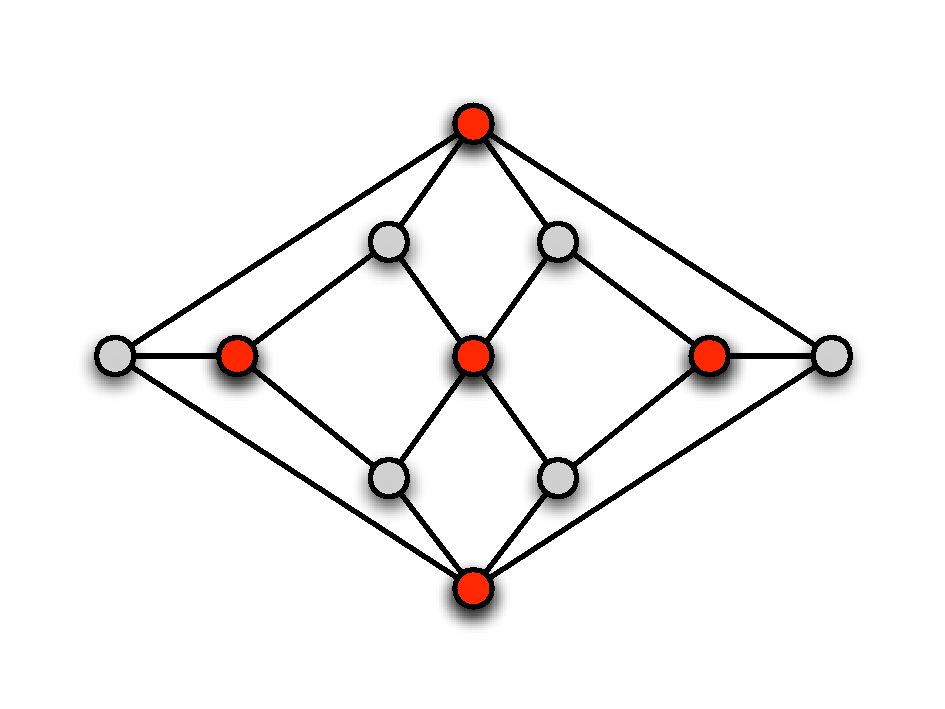
\includegraphics[width=10cm]{pic1.pdf}
    \end{center}
\caption{Herschelov graf, vektorska grafika.}
\label{pic1}
\end{figure}
Pa res lahko vključimo slike katerihkoli formatov? Žal ne. Programski paket \LaTeX\ lahko uporabljamo v več dialektih. Ukaz {\tt latex} ne mara vključenih slik v formatu Portable Document Format {\tt .pdf}, ukaz {\tt pdflatex} pa ne prebavi slik v Encapsulated Postscript Formatu {\tt .eps}.
Strnjeno v Tabeli~\ref{tbl:1}.

\begin{table}
\caption{}
    \begin{center}
        \begin{tabular}{l|ccc}
            ukaz/format & {\tt .pdf} & {\tt .eps} & ostali formati \\ \hline
                        {\tt pdflatex} & da & ne & da \\
                        {\tt latex}   & ne & da  & da
        \end{tabular}
    \end{center}
\label{tbl:1}
\end{table}

Nasvet? Odločite se za uporabo ukaza {\tt pdflatex}. Vaš izdelek bo brez vmesnih stopenj na voljo v {.pdf} formatu in ga lahko odnesete v vsako tiskarno. Če morate na vsak način vključiti sliko, ki jo imate v {\tt .eps} formatu, jo vnaprej pretvorite v alternativni format, denimo {\tt .pdf}.

Včasih se da v okolju za uporabo programskega paketa \LaTeX\ nastaviti na kakšen način bomo prebavljali vhodne dokumente. Spustni meni na Sliki~\ref{pic2} odkriva uporabo \LaTeX{}a v njegovi pdf inkarnaciji --- {\tt pdflatex}.
\begin{figure}
\begin{center}

\includegraphics[width=10cm]{pic2.png}
\end{center}
\caption{Kateri dialekt uporabljati?}
\label{pic2}
\end{figure}
Vključena Slika~\ref{pic2} je seveda bitna.



%----------------------------------------------------------------
% Poglavje (Chapter) 4
%----------------------------------------------------------------
\chapter{Razno}
\label{ch:razno}

\section{Notacije}
\label{sec:notacije}

Za notacijo spremenljivk ter skalarjev uporabimo običajno notacijo, t.j., spremenljivka $x$ in skalar $a$. Pri notaciji matrik ter vektorjev pa se poslužujemo krepega fonta. Torej, matrika $\boldsymbol{A}$ ter vektor $\boldsymbol{v}$,
\begin{equation}
\boldsymbol{A} = \begin{bmatrix}
       a_{11} & a_{12} & \dots & a_{1q}  \\
       a_{21} & a_{22} & \dots & a_{2q}  \\
       \vdots  \\
       a_{p1} & a_{p2} & \dots & a_{pq}  \\
     \end{bmatrix}, \quad
     \boldsymbol{v} = \begin{bmatrix}
       x_1  \\
       x_2  \\
       \vdots  \\
       x_q  \\
     \end{bmatrix}. \nonumber
\end{equation}

%----------------------------------------------------------------
\section{Lepe tabele in psevdokoda}
\label{sec:psevdokoda}

Psevdokoda~\ref{alg:primer} prikazuje primer delovanja genetskega algoritma, medtem ko Tabela~\ref{tab:params} prikazuje primer lepe tabele brez vertikalnih črt.

\begin{algorithm}
\caption{Psevdokoda genetskega algoritma}
\label{alg:primer}
\begin{algorithmic}[1]
\footnotesize
\STATE $t \gets 0$
\STATE $InitPopulation[P(t)] \gets$ inicializiraj populacijo
\STATE $EvalPopulation[P(t)] \gets$ evaluiraj populacijo
\REPEAT
\STATE $P'(t) \gets Variation[P(t)] \gets $ generiraj novo populacijo
\STATE $EvalPopulation[P'(t)] \gets$ evaluiraj novo populacijo
\STATE $P(t+1) \gets ApplyGeneticOperators[P'(t) \in Q]$
\STATE $t \gets t+1$
\UNTIL{prekinitev}
\IF{rezultat dovolj dober}
\STATE shrani rezultat
\ENDIF
\end{algorithmic}
\end{algorithm}

%---------------------------------------------------------------
\begin{table}
\caption{Primer enostavne tabele.}
\centering
\scalebox{0.82}{
\begin{tabular}{c c c}
 \toprule
 Ime & Vrednost & Opis \\
 \midrule
 \textit{ $a$ } & 0.03 &  skalar \\
 \textit{ $x$ } & -1 & spremenljivka \\
 \bottomrule
\end{tabular}
}
\label{tab:params}
\end{table}

%----------------------------------------------------------------
% Poglavje (Chapter) 5
%----------------------------------------------------------------
\chapter{Kaj pa literatura?}
\label{ch3}
Kot smo omenili že v uvodu, je pravi način za citiranje literature uporaba \BibTeX{}a~\cite{ubi}.
Programski paket \LaTeX je prvotno predstavljen v priročniku~\cite{Lamport} in je v resnici nadgradnja sistema \TeX\ avtorja Donalda Knutha, znanega po denimo, če izpustim njegovo umetnost programiranja, Knuth-Bendixovem algoritmu~\cite{Knuth}.

Vsem raziskovalcem s področja računalništva pa svetujem v branje mnenje L.\ Fortnowa~\cite{Fortnow}.

%----------------------------------------------------------------
% Poglavje (Opis funkciionalnosti) 5
%----------------------------------------------------------------
\chapter{Opis funkcionalnosti}
\label{ch4}
\section{Prepoznavanje imenskih entitet}
\label{sec:ner}
Prepoznavanje imenskih entitet je tehnika na področju obdelave naravnega jezika, ki se uporablja za prepoznavanje in klasifikacijo besed v besedilu. Te posebne vrste so imenovane entitete, kot so imena oseb, organizacij, lokacij, datumov, številk, denarnih zneskov in drugih specifičnih poimenovanj.

Cilj je prepoznati in določiti začetek in konec posameznih entitet v besedilu ter jim pripisati ustrezno kategorijo. Na primer, v stavek "Janez Novak je rojen 10. avgusta 1985 v Ljubljani" bi sistem prepoznal "Janez Novak" kot ime osebe, "10. avgust 1985" kot datum in "Ljubljana" kot lokacijo.

Številne praktične uporabe:
\begin{enumerate}
 \item  Avtomatsko označevanje imenskih entitet v novicah, člankih in drugih besedilnih vsebinah.
 \item Razumevanje strukture in vsebine dokumentov za informacijsko iskanje in kategorizacijo.
 \item Pomoč pri analizi sentimenta, kjer se želimo razumeti, kako se osebe, organizacije ali druge entitete omenjene v besedilu nanašajo na določeno temo ali izdelek.
\end{enumerate}

\section{Analiza sentimenta}
Analiza sentimenta je proces določanja čustvenega odziva, nagnjenosti ali stališča zapisanega besedila. Cilj analize sentimenta je ugotoviti, ali je določeno besedilo pozitivno, negativno ali nevtralno. To je lahko koristno pri analizi mnenj strank, razumevanju čustvenega odziva na izdelke, blagovne znamke, dogodke in druge.
Na primer, če imamo naslednji stavek: "Ta film je fantastičen, vreden ogleda!", bi analiza sentimenta prepoznala, da je izraz pozitiven.
Ta analiza temelji na uporabi naravnojezikovnega procesiranja in strojnega učenja. Obstaja več pristopov k analizi sentimenta, vključno z naslednjimi:
\begin{enumerate}
 \item Pravilni pristopi: Uporabljajo se predvsem pravila in vzorci za identifikacijo pozitivnih in negativnih izrazov v besedilu. Na primer, besede, kot so "dobro", "fantastično", "radostno" itd., bi bile označene kot pozitivne, medtem ko bi bile besede, kot so "slabo", "žalostno", "neznosno" itd., označene kot negativne.
 \item Strojno učenje na podlagi besedila: Ta pristop vključuje uporabo algoritmov strojnega učenja, ki so naučeni prepoznati čustveni naboj besed v besedilu na podlagi velikega števila označenih podatkov (besedil s čustvenimi oznakami). 
 \item Analiza sentimenta s čustvenimi slovarji: Ta pristop vključuje uporabo slovarjev z besedami in izrazoslovjem, ki so povezani z določenimi čustvi. Besedilo se nato preveri in oceni glede na prisotnost pozitivnih ali negativnih besed iz čustvenih slovarjev.
 \item Algoritmi globokega učenja: V zadnjem času so se pojavili tudi pristopi, ki temeljijo na globokem učenju.
 \end{enumerate}
 
 \section{Povzemanje besedila}
Pri povzermanju besedila gre za postopek ustvarjanja krajšega in jedrnatega povzetka izdaljšega besedila, kot je članek ali dokument. Namen povzemanja je izluščiti ključne informacije in ideje iz izvornega besedila ter jih predstaviti na bolj pregleden in krajši način. To je zelo koristno v velikih količinah podatkov, ko želimo hitro pridobiti bistvo informacij, ne da bi brali celotno besedilo.

NLP tehnike za povzemanje uporabljajo različne algoritme in metode, ki vključujejo strojno učenje in obdelavo naravnega jezika, da bi učinkovito izluščile ključne besede, stavke ali odstavke, ki predstavljajo osrednje ideje v izvornem besedilu. Rezultat je običajno kratek povzetek, ki ohranja pomembne informacije iz izvirnega besedila. Ta tehnologija ima širok spekter uporab, kot so samodejno povzemanje novic, generiranje opisov izdelkov, izdelava povzetkov raziskovalnih člankov in še veliko več.
 
 \section{Izvleček besedne zveze}
Nanaša se na besede ali izraze, ki so najpomembnejši ali najbolj značilni za določeno besedilo ali dokument. Te besede so običajno tiste, ki nosijo ključne informacije ali so bistvene za razumevanje vsebine.

Identifikacija ključnih besed je pomembna naloga, saj nam omogoča, da hitro ugotovimo, o čem govori določen tekst. Te besede so lahko uporabne tudi za avtomatsko indeksiranje dokumentov, iskanje relevantnih informacij in razumevanje teme besedila brez potrebe po branju celotnega besedila.

 \section{Klasifikacija besedila}
 Klasifikacija besedil je tehnika, pri kateri avtomatizirano določimo kategorijo ali razred določenega besedila na podlagi vsebine besedila. To je lahko zelo uporabno, saj nam omogoča razvrščanje besedil v različne skupine glede na njihovo vsebino. Na primer, lahko klasificiramo e-poštna sporočila kot "spam" ali "ne-spam", novice glede na tematiko, uporabniške komentarje glede na ton (pozitiven, negativen, nevtralen), itd.

Postopek klasifikacije besedil se običajno začne s pripravo in čiščenjem besedil. To vključuje odstranjevanje nepotrebnih znakov, šumnikov, posebnih znakov, pretvorbo vseh črk v male črke, lahko pa tudi odstranjevanje pogostih besed, ki nimajo velikega pomena za klasifikacijo (npr. "in", "ali", "je", "na", "s", itd.).

Nato se besedila predstavijo v obliki, ki jo lahko uporabimo za učenje modela. Pogosto se uporablja metoda imenovana vreča besed ("Bag-of-Words"), kjer se besedilo pretvori v nabor besed, ki se pojavljajo v njem, in število pojavitev teh besed. Ta postopek lahko ponazorimo s pomočjo vektorja.
 
  \section{Zaznava objektov}
Je tehnika, ki se uporablja za avtomatsko zaznavanje in identifikacijo objektov na digitalnih slikah ali video posnetkih. Namen te tehnike je, da  prepozna in označi različne objekte v podobi ter jih loči od ozadja ali drugih objektov.

Postopek objektnega zaznavanja običajno vključuje naslednje korake:
\begin{enumerate}
 \item Zaznavanje: Model preučuje sliko ali video posnetek in identificira regije, kjer bi se lahko nahajali objekti.
 \item Lokalizacija: Po tem, ko so bile regije prepoznane, algoritem določi omejitveno okvirje (bounding boxes), ki natančno označujejo položaje in mejne točke objektov na sliki.
 \item Klasifikacija: Ko so objekti omejeni z omejitvenimi okviri, analizira vsebino znotraj teh okvirov in jih razvrsti v različne kategorije (npr. avto, pes, zgradba, itd.).
 \item  Sledenje: V video posnetkih je lahko zaželeno, da algoritem sledi objektom skozi različne kadre in tako beleži njihovo gibanje.
 \end{enumerate}
Objektno zaznavanje se uporablja v številnih aplikacijah, kot so samovozeča vozila za zaznavanje drugih vozil in pešcev, nadzorne kamere za varnostne namene, prepoznavanje obrazov, identifikacija prometnih znakov, analiza medicinskih slik in še veliko drugega. Gre za enega ključnih elementov umetne inteligence. %----------------------------------------------------------------
% Poglavje (Uporabljeni dataseti) 6
%----------------------------------------------------------------
\chapter{Dataseti}
\label{ch5}
\section{Kaj je dataset?}
Dataset je zbirka podatkov, ki so organizirani in shranjeni v strukturirani ali ne-strukturirani obliki ter označeni za namen analize, raziskav, učenja modelov ali drugih postopkov obdelave podatkov. Dataseti vsebujejo različne vrste podatkov, od številk, besedil, slik, zvokov, videoposnetkov do drugih tipov informacij.
V kontekstu računalniškega znanstvenega modeliranja in strojnega učenja so dataseti ključnega pomena, saj služijo kot osnova za razvoj, treniranje in evalvacijo modelov. Modeli se učijo na teh podatkih, tako da prepoznajo vzorce in povezave med vhodnimi podatki in ciljnimi izhodi.
Na primer, v naravnojezikovni obdelavi  dataset vsebuje besedilne podatke, ki so lahko članki, knjige, novičarski članki ali socialni mediji. Te podatke lahko uporabimo za različne naloge, kot je sentimentna analiza, klasifikacija tem, generiranje besedil itd.
V poslovnem okolju se dataseti uporabljajo za analizo strank, trženjske kampanje, obdelavo naravnega jezika v storitvah za stranke in še veliko drugih aplikacij.
Pomembno je, da so dataseti pravilno pripravljeni, imajo ustrezne metapodatke in so primerni za ciljno nalogo, da bi omogočili kakovostno analizo in doseganje uporabnih rezultatov.

\section{Uporabljeni dataseti}
\subsection{CoNLL 2003}
\label{sec:my_subsection}
 Je zbirka podatkov, ki se uporablja za razvoj in evalvacijo sistemov za obdelavo naravnega jezika , zlasti za nalogo imenovanja imenovalnih entitet.  Imenuje se po konferenci CoNLL (Conference on Computational Natural Language Learning) leta 2003, kjer je bil ta nabor podatkov predstavljen v okviru tekmovanja za prepoznavanje imenovanih entitet.
 Dataset CoNLL 2003 je priljubljen referenčni dataset za prepoznavanje poimenovanih entitet naravnega jezika v obdelavi naravnega jezika. Uporabljen je bil v skupni nalogi na konferenci o računalniškem učenju naravnega jezika (CoNLL) leta 2003.

 \begin{figure}[h!]
\begin{center}
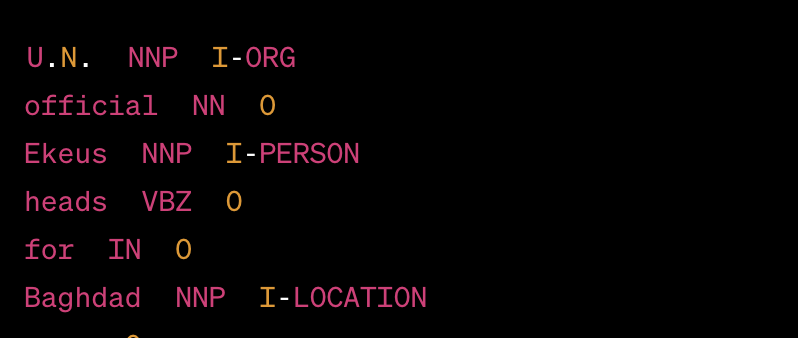
\includegraphics[width=10cm]{conll.png}
\end{center}
\caption{CoNLL2003 dataset}
\label{pic2}
\end{figure}

Poimenovane entitete so razdeljene v štiri glavne kategorije:
\begin{enumerate}
 \item Oseba (PER): Posamezna imena ljudi.
 \item Organizacija (ORG): Imena podjetij, ustanov ali organizacij.
 \item Lokacija (LOC): Imena geografskih lokacij, kot so mesta, države ali regije.
 \item Razno (MISC): Druge poimenovane entitete, ki ne spadajo v zgoraj navedene kategorije, na primer datumi, odstotki ali denar.
 \end{enumerate}
 Podatki v datasetu so predstavljeni v obliki ene besede na vrstico, kjer vsaka vrstica predstavlja besedo in pripadajočo oznako v stavku. Besede in oznake so ločene z belim prostorom.
 Dataset CoNLL 2003 se pogosto uporablja za evalvacijo zmogljivosti modelov za prepoznavanje poimenovanih entitet in že več let je standardni benchmark za raziskovalce in strokovnjake v skupnosti obdelave naravnega jezika. Ostaja dragocen vir za razvoj in preizkušanje novih algoritmov in sistemov za NER.
Dataset je sestavljen/razdeljen na tri različne skupine in sicer:
CoNLL2003  podatkovna zbirka je običajno razdeljena na tri sklope:
\begin{enumerate}
 \item učni (train) z 14.000 vrsticami  primerov
 \item validacijski (validation) z 3.250 vrsticami primerov
 \item preizkusni (test) z 3.450 vrsticami primerov
 \end{enumerate}

\subsection{IMDb Reviews dataset}
\label{sec:imdb}
IMDB podatkovna zbirka, znana tudi kot IMDB Movie Reviews Dataset, je priljubljen benchmark podatkovni niz v področju obdelave naravnega jezika. Ta niz je sestavljen iz pregledov filmov, ki so jih prispevali uporabniki na spletni strani IMDb (Internet Movie Database).

Podatki vsebujejo ocene in besedilne komentarje, ki jih je ustvarila skupnost uporabnikov IMDb. Vsak pregled vsebuje besedilni komentar in oceno filma, ki se giblje med 1 (najslabša) in 10 (najboljša). Cilj te podatkovne zbirke v naravnem jeziku je razviti modele, ki lahko avtomatsko analizirajo besedilne komentarje in napovedo, ali je pregled pozitiven ali negativen glede na oceno in besedilo.
IMDB podatkovna zbirka je običajno razdeljena na dva sklopa: 
\begin{enumerate}
 \item učni (train) z 25.000 vrsticami  primerov
 \item preizkusni (test) z 25.000 vrsticami primerov
 \end{enumerate}
Vsak sklop vsebuje tisoče pregledov filmov. To je idealna podatkovna zbirka za naloge analize čustvenega tona besedil (sentiment analysis), kjer modeli ocenjujejo, ali je mnenje v besedilu pozitivno, negativno ali nevtralno.

\subsection{ COCO dataset}
\label{sec:coco}
COCO (Common Objects in Context) je široko uporabljen nabor podatkov v področju računalniškega vida in detekcije objektov. Namenjen je zagotavljanju celovite in raznolike zbirke slik za različne naloge, vključno z detekcijo objektov, segmentacijo in podnaslavljanjem. Nabor podatkov naj bi odražal scenarije iz resničnega sveta in vsebuje slike, ki so kompleksne ter vključujejo več objektov v različnih kontekstih.

Nabor podatkov COCO je obsežen in vsebuje deset tisoče slik z milijoni označenih posameznih objektov. Slike prihajajo iz različnih virov, zajemajo raznolike prizore, ozadja, svetlobne pogoje in velikosti objektov.


Tukaj je nekaj ključnih značilnosti nabora podatkov COCO:
\begin{enumerate}
 \item Kategorije slik: Nabor podatkov COCO vsebuje slike, ki zajemajo 80 različnih kategorij objektov, od splošnih objektov, kot so "oseba," "avto" in "pes," do bolj specifičnih objektov, kot so "mobilni telefon," "zobna ščetka" in "zmaj."

 \item Anotacije: Vsaka slika v naboru podatkov COCO je opremljena z oznakami na ravni objekta in koordinatami  okvirja. To pomeni, da je vsak posamezen objekt določene kategorije znotraj slike označen, okoli njega pa je narisano območje z okvirjem, ki označuje njegovo lokacijo. Informacije o anotacijah so ključnega pomena za usposabljanje modelov za detekcijo objektov in segmentacijo.

 \item Segmentacija objektov: Poleg anotacij območja z okviri nabor podatkov COCO prav tako zagotavlja maske segmentacije na ravni slikovnih pik za vsak posamezen objekt. To pomeni, da so objekti ne le lokalizirani z okviri, ampak so natančno določene tudi meje objektov na ravni slikovnih pik.

 \item Izzivi in tekmovanja: Nabor podatkov COCO je spodbudil številne izzive in tekmovanja v skupnosti računalniškega vida. COCO izziv je priljubljen dogodek, na katerem raziskovalci in inženirji predstavijo svoje modele za detekcijo objektov, segmentacijo in podnaslavljanje, s čimer premikajo meje tega, kar je mogoče v teh področjih.
 \end{enumerate}
 COCO podatkovna zbirka je običajno razdeljena na dva sklopa: 
\begin{enumerate}
 \item učni (train) z 117.000 primeri
 \item preizkusni (test) z 4.950 primeri
 \end{enumerate}
 
 \subsection{ CNN/Daily Mail Dataset}
 \label{sec:cnn}
 CNN/Daily Mail je zbirka novičarskih člankov skupaj s povzetki, ki se uporablja za usposabljanje in preizkušanje modelov za avstraktivno povzemanje besedil. Ta nabor podatkov vsebuje različne novičarske članke in njihove povzetke, zaradi česar je primeren za naloge avstraktivnega povzemanja, kjer se ustvarijo povzetki v lastnih besedah, ne le izbirajo stavke iz izvornega besedila.
 Nabor podatkov vsebuje na tisoče člankov s pripadajočimi povzetki, kar omogoča raziskovalcem obsežno usposabljanje in preizkušanje modelov.
 Tukaj je nekaj ključnih značilnosti nabora podatkov CNN/Daily Mail:
 \begin{enumerate}
  \item Novičarski Članki in Povzetki: Nabor podatkov vsebuje novičarske članke iz medijskih virov, kot sta CNN (Cable News Network) in Daily Mail, skupaj s pripadajočimi povzetki. Ti članki pokrivajo različne teme in dogodke ter so različnih dolžin.
 \item Avstraktivno Povzemanje: Za razliko od ekstraktivnega povzemanja, kjer se izvlečejo in združijo stavki iz izvornega besedila, avstraktivno povzemanje vključuje ustvarjanje povzetka v povsem novih besedah. Nabor podatkov CNN/Daily Mail je priljubljen za tovrstno naloge avstraktivnega povzemanja.
  \end{enumerate}
CNN/Daily Mail podatkovna zbirka je običajno razdeljena na tri sklope: 
\begin{enumerate}
 \item učni (train) z 287.000 vrsticami  primerov
 \item validacijski (validation) z 13.400 vrsticami primerov
 \item preizkusni (test) z 11.500 vrsticami primerov
 \end{enumerate}
 
 \subsection{ semeval-2017 dataset}
  \label{sec:semeval}
 SemEval podatkovne zbirke so zbirke besedilnih podatkov, ki so anotirane za različne naloge na področju obdelave naravnega jezika.
 
Tukaj je nekaj ključnih značilnosti SemEval podatkovnih zbirk:
\begin{enumerate}
 \item Anotacije: Podatki v SemEval podatkovnih zbirkah so običajno anotirani, kar pomeni, da so označeni z dodatnimi informacijami. Na primer, v podatkovni zbirki za naloge razreševanja sentimenta bi bili vzorci besedil označeni s pozitivnimi, negativnimi ali nevtralnimi sentimenti.

 \item Naloge: Vsaka SemEval podatkovna zbirka je oblikovana za reševanje specifične naloge naravnega jezika. To lahko vključuje naloge, kot so analiza sentimenta, prepoznavanje imenovanih entitet, razreševanje koreference, klasifikacija besedil itd.

 \item Raznolikost: SemEval podatkovne zbirke zajemajo širok spekter nalog, jezikov in domen. To omogoča raziskovalcem primerjavo modelov in pristopov na različnih področjih.

 \item Uporaba v tekmovanjih: SemEval podatkovne zbirke se pogosto uporabljajo v tekmovanjih, imenovanih SemEval naloge. Tekmovalci tekmujejo za razvoj najboljših algoritmov za določeno nalogo in se primerjajo z drugimi udeleženci.
 \end{enumerate}
Raziskovalna skupnost: SemEval podatkovne zbirke so postale pomemben del naravnega jezika raziskovalne skupnosti, saj omogočajo primerjavo najnovejših pristopov in tehnologij na enotnem naboru podatkov.
SemEval  podatkovna zbirka je običajno razdeljena na tri sklope: 
\begin{enumerate}
 \item učni (train) z 49.547 vrsticami  primerov
 \item validacijski (dev) z 12.285 vrsticami primerov
 \item preizkusni (test) z 12.285 vrsticami primerov
 \end{enumerate}
 
 %----------------------------------------------------------------
% Poglavje (Uporabljeni dataseti) 6
%----------------------------------------------------------------
\chapter{Dataseti}
\label{ch5}
\section{Metrike}
\subsection{Opis spremelnjivk za izračun metrik}
\textbf{Pravilno pozitivni (True Positive)}

Je izraz, ki se uporablja v statistiki in strojnem učenju za opis primerov, kjer je model pravilno napovedal pozitiven rezultat za določen razred. To pomeni, da je model prepoznal pozitiven pojav, ko je bil dejansko prisoten.

\emph{Primer:}

Predpostavimo, da razvijamo model za prepoznavanje spam sporočil v elektronski pošti. Model pravilno prepozna 25 sporočil kot nezaželena (spam), ki dejansko vsebujejo nezaželeno vsebino. To pomeni, da imamo 25 primerov "pravih pozitivnih". Te primere model pravilno prepozna kot spam, ker resnično vsebujejo neželeno vsebino.



\textbf{Napačno pozitivni (False Positive)}

Označuje situacijo, ko model napačno napove, da je nekaj pozitivno, medtem ko je v resnici negativno. Gre za vrsto napake, kjer model napačno identificira primer kot pripadajoč pozitivnemu razredu, čeprav dejansko pripada negativnemu razredu.


\emph{Primer:}

Predpostavimo, da imamo model za prepoznavanje spam sporočil v elektronski pošti. Če model označi sporočilo kot "spam", čeprav ni dejansko spam, imamo situacijo lažno pozitivnega primera. Drugače povedano, model je napačno napovedal pozitiven primer (spam), ko je dejansko negativen primer (ni spam).


\textbf{Napačno negativni (False Negatives)}

Označuje napako, ki se pojavi v kontekstu klasifikacije ali analize besedila, ko model napačno napove, da je nekaj negativno, čeprav je v resnici pozitivno. To je vrsta napake, kjer model spregleda ali ne prepozna pozitivnih primerov.

V primeru analize besedila v naravni jezikovni obdelavi (NLP), false negative se zgodi, ko model ne uspe zaznati pozitivnega elementa v besedilu, ki bi ga moral prepoznati. Na primer, če imamo model za prepoznavanje pozitivnih izjav v komentarjih in model spregleda pozitivno izjavo, to bi bil primer false negative.

\emph{Primer:}


Predpostavimo, da imamo napreden sistem za filtriranje neželenih sporočil (spam), ki ga uporabljamo za preverjanje prihajajočih e-poštnih sporočil. Sistem je zasnovan tako, da prepoznava in premika neželena sporočila v mapo za neželeno pošto.

Vendar pa se zgodi False Negative, ko sistem napačno presodi e-poštno sporočilo kot varno (ne-spam), čeprav vsebuje vse znake neželene vsebine. Na primer, če e-poštno sporočilo vsebuje povezave do nerealnih ponudb ali oglasev za sumljive izdelke, bi bila takšna sporočila številčno gledano ena od "False Negatives".

V tem primeru je sistem spregledal prepoznavo neželene vsebine, kar je povzročilo, da je sporočilo pristalo v glavnem predalu prejete pošte namesto v mapi za neželeno pošto. To lahko predstavlja težavo, saj se takšni neželeni vsebini lahko izognemo le, če sistem zanesljivo prepozna vse takšne primere.


\subsection{Precision}

Precision je pomembna metrika za ocenjevanje uspešnosti modelov v različnih nalogah, kot je klasifikacija, kjer se ukvarjamo z razdelitvijo podatkov v različne razrede. Poudarja natančnost pozitivnih napovedi, torej tistih primerov, ki jih model prepozna kot pozitivne. Visoka preciznost pomeni, da so pozitivne napovedi modela zanesljive in imajo malo lažno pozitivnih napak.

V kontekstu naravne jezikovne obdelave (NLP), precision igra ključno vlogo pri razumevanju besedila. Na primer, pri analizi sentimenta želimo natančno ugotoviti, ali je izraz pozitiven ali negativen. Visoka preciznost v tem primeru pomeni, da so napovedi modela o sentimentu točne in se malo zmotijo.

 
 Formula za izračun:
\begin{center}
 Precision = \(\frac{True Positive}{True Positive + False Negatives}\)
\end{center}

 Povzeto po:https://www.analyticsvidhya.com/blog/2021/07/metrics-to-evaluate-your-classification-model-to-take-the-right-decisions/

\subsection{Recall}
Nanaša se na eno od metrik uspešnosti pri vrednotenju modelov za obdelavo naravnega jezika. Recall se meri kot razmerje med številom pravilno prepoznanih relevantnih primerov in celotnim številom dejansko obstoječih relevantnih primerov. Višji recall pomeni, da je model bolje usposobljen za iskanje in pridobivanje vseh relevantnih informacij, vendar to lahko vodi tudi v več lažno pozitivnih rezultatov. Zato je pomembno doseči uravnoteženost med recallom in natančnostjo (precision) pri oceni uspešnosti modelov. Primer uporabe recalla  je v iskalnih sistemih, kjer želimo zagotoviti, da se relevantni dokumenti ali informacije ne izpustijo pri iskanju. S pravilno optimizacijo modelov lahko dosežemo visoko kakovostno izluščevanje informacij iz besedil, kar je ključno za številne aplikacije, kot so avtomatizirano odzivanje na povratne informacije strank, analiza sentimenta in razumevanje besedil v različnih jezikih.

 Formula za izračun:
\begin{center}
 Recall = \(\frac{True Positive}{True Positive + False Positive}\)
\end{center}

\subsection{F1}

F1-metrika je pomembna za ocenjevanje uspešnosti modelov v obdelavi besedil in naravnojezikovnem procesiranju. Združuje oceni natančnosti (precision) in prepoznavnosti (recall) v eno številko, ki odraža ravnotežje med temi dvema metrikama. Pri NLP nalogah, kot so klasifikacija besedil, izluščanje informacij ali identifikacija entitet, sta tako natančnost kot prepoznavnost ključni. Visoka natančnost pomeni pravilno identifikacijo relevantnih elementov, medtem ko visok recall zagotavlja prepoznavanje vseh resnično pozitivnih primerov. F1-metrika se izračuna kot povprečje med natančnostjo in prepoznavnostjo, dajeta pa ji enako težo. To omogoča, da ocenimo, kako dobro model obvladuje oba cilja hkrati. Visoka vrednost F1-metrike kaže, da je model uspešno uskladil identifikacijo pravih pozitivnih primerov z izogibanjem napačno pozitivnim rezultatom. Uporaba F1-metrike je zlasti smiselna, ko sta natančnost in prepoznavnost pomembni za končni rezultat in ko želimo doseči optimalno uravnoteženost med tema dvema vidikoma.


 Formula za izračun:
\begin{center}
 F1 = 2 x \(\frac{Precision \times Recal}{Precision + Recal}\)
\end{center}

\subsection{Accuracy}
\subsection{ROUGE}



  %----------------------------------------------------------------
% Poglavje (Uporabljeni dataseti) 6
%----------------------------------------------------------------
\chapter{Analiza raziskave}
\subsection{Prepoznavanje imenskih entitet (Named Entity Recognition)}
\begin{table}[h!]
\caption{Prepoznavanje imenskih entitet}
        \begin{tabular}{l|ccc}
             & {\tt Precision} & {\tt Recall}  & F1   \\ \hline
                        {\tt Transformers} & 0.949 & 0.953 & 0.951 \\
                        {\tt Vertex AI }   & 0.920 & 0.919  & 0.919  \\
                         {\tt AWS SageMaker}   & \textbf {0.954} & \textbf {0.961}& \textbf {0.958}  \\     
                        {\tt Azure Cognitive Services}   & 0.858 & 0.824  & 0.840
        \end{tabular}
\label{tbl:1}
\end{table}

 \begin{figure}[h!]
\begin{center}
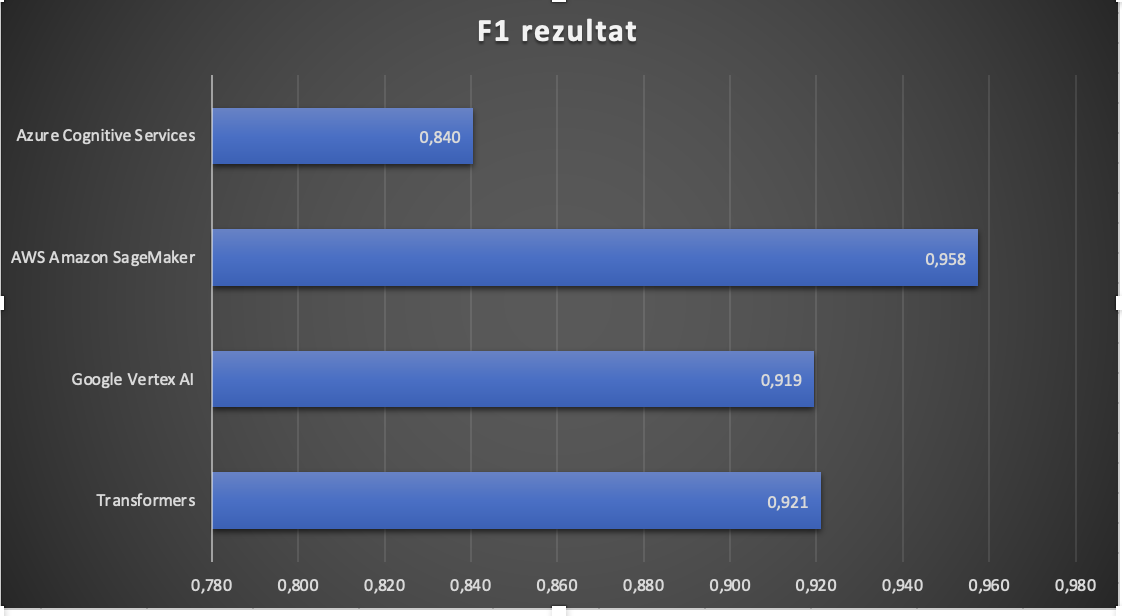
\includegraphics[width=8cm]{NER.png}
\end{center}
\caption{Prepoznavanje imenskih entitet F1 rezultat}
\label{pic2}
\end{figure}
Pri analizi imenskih entitet je bil uporabljen \hyperref[sec:my_subsection]{\underline {CONLL-2003}} dataset.

Za prepoznavanje oseb (PER) in organizacij (ORG) se je najbolje izkazal Vertex AI storitev. Na splošno pa je bil v vseh področjih najboljši AWS SageMaker storitev.

\subsection{Analiza sentimenta (Sentiment Analaysis)}
\begin{table}[h!]
\caption{Analiza sentimenta}
        \begin{tabular}{l|ccc}
             & {\tt Precision} & {\tt Recall}  & F1   \\ \hline
                        {\tt Transformers} & 0.800 & 0.799 & 0.799 \\
                        {\tt Vertex AI }   & \textbf {0.924} & \textbf {0.924 } & \textbf {0.924}  \\
                         {\tt AWS SageMaker}   & 0.862 & 0.891 & 0.876 \\     
                        {\tt Azure Cognitive Services}   & 0.862 & 0.891  & 0.877
        \end{tabular}
\label{tbl:1}
\end{table}

 \begin{figure}[h!]
\begin{center}
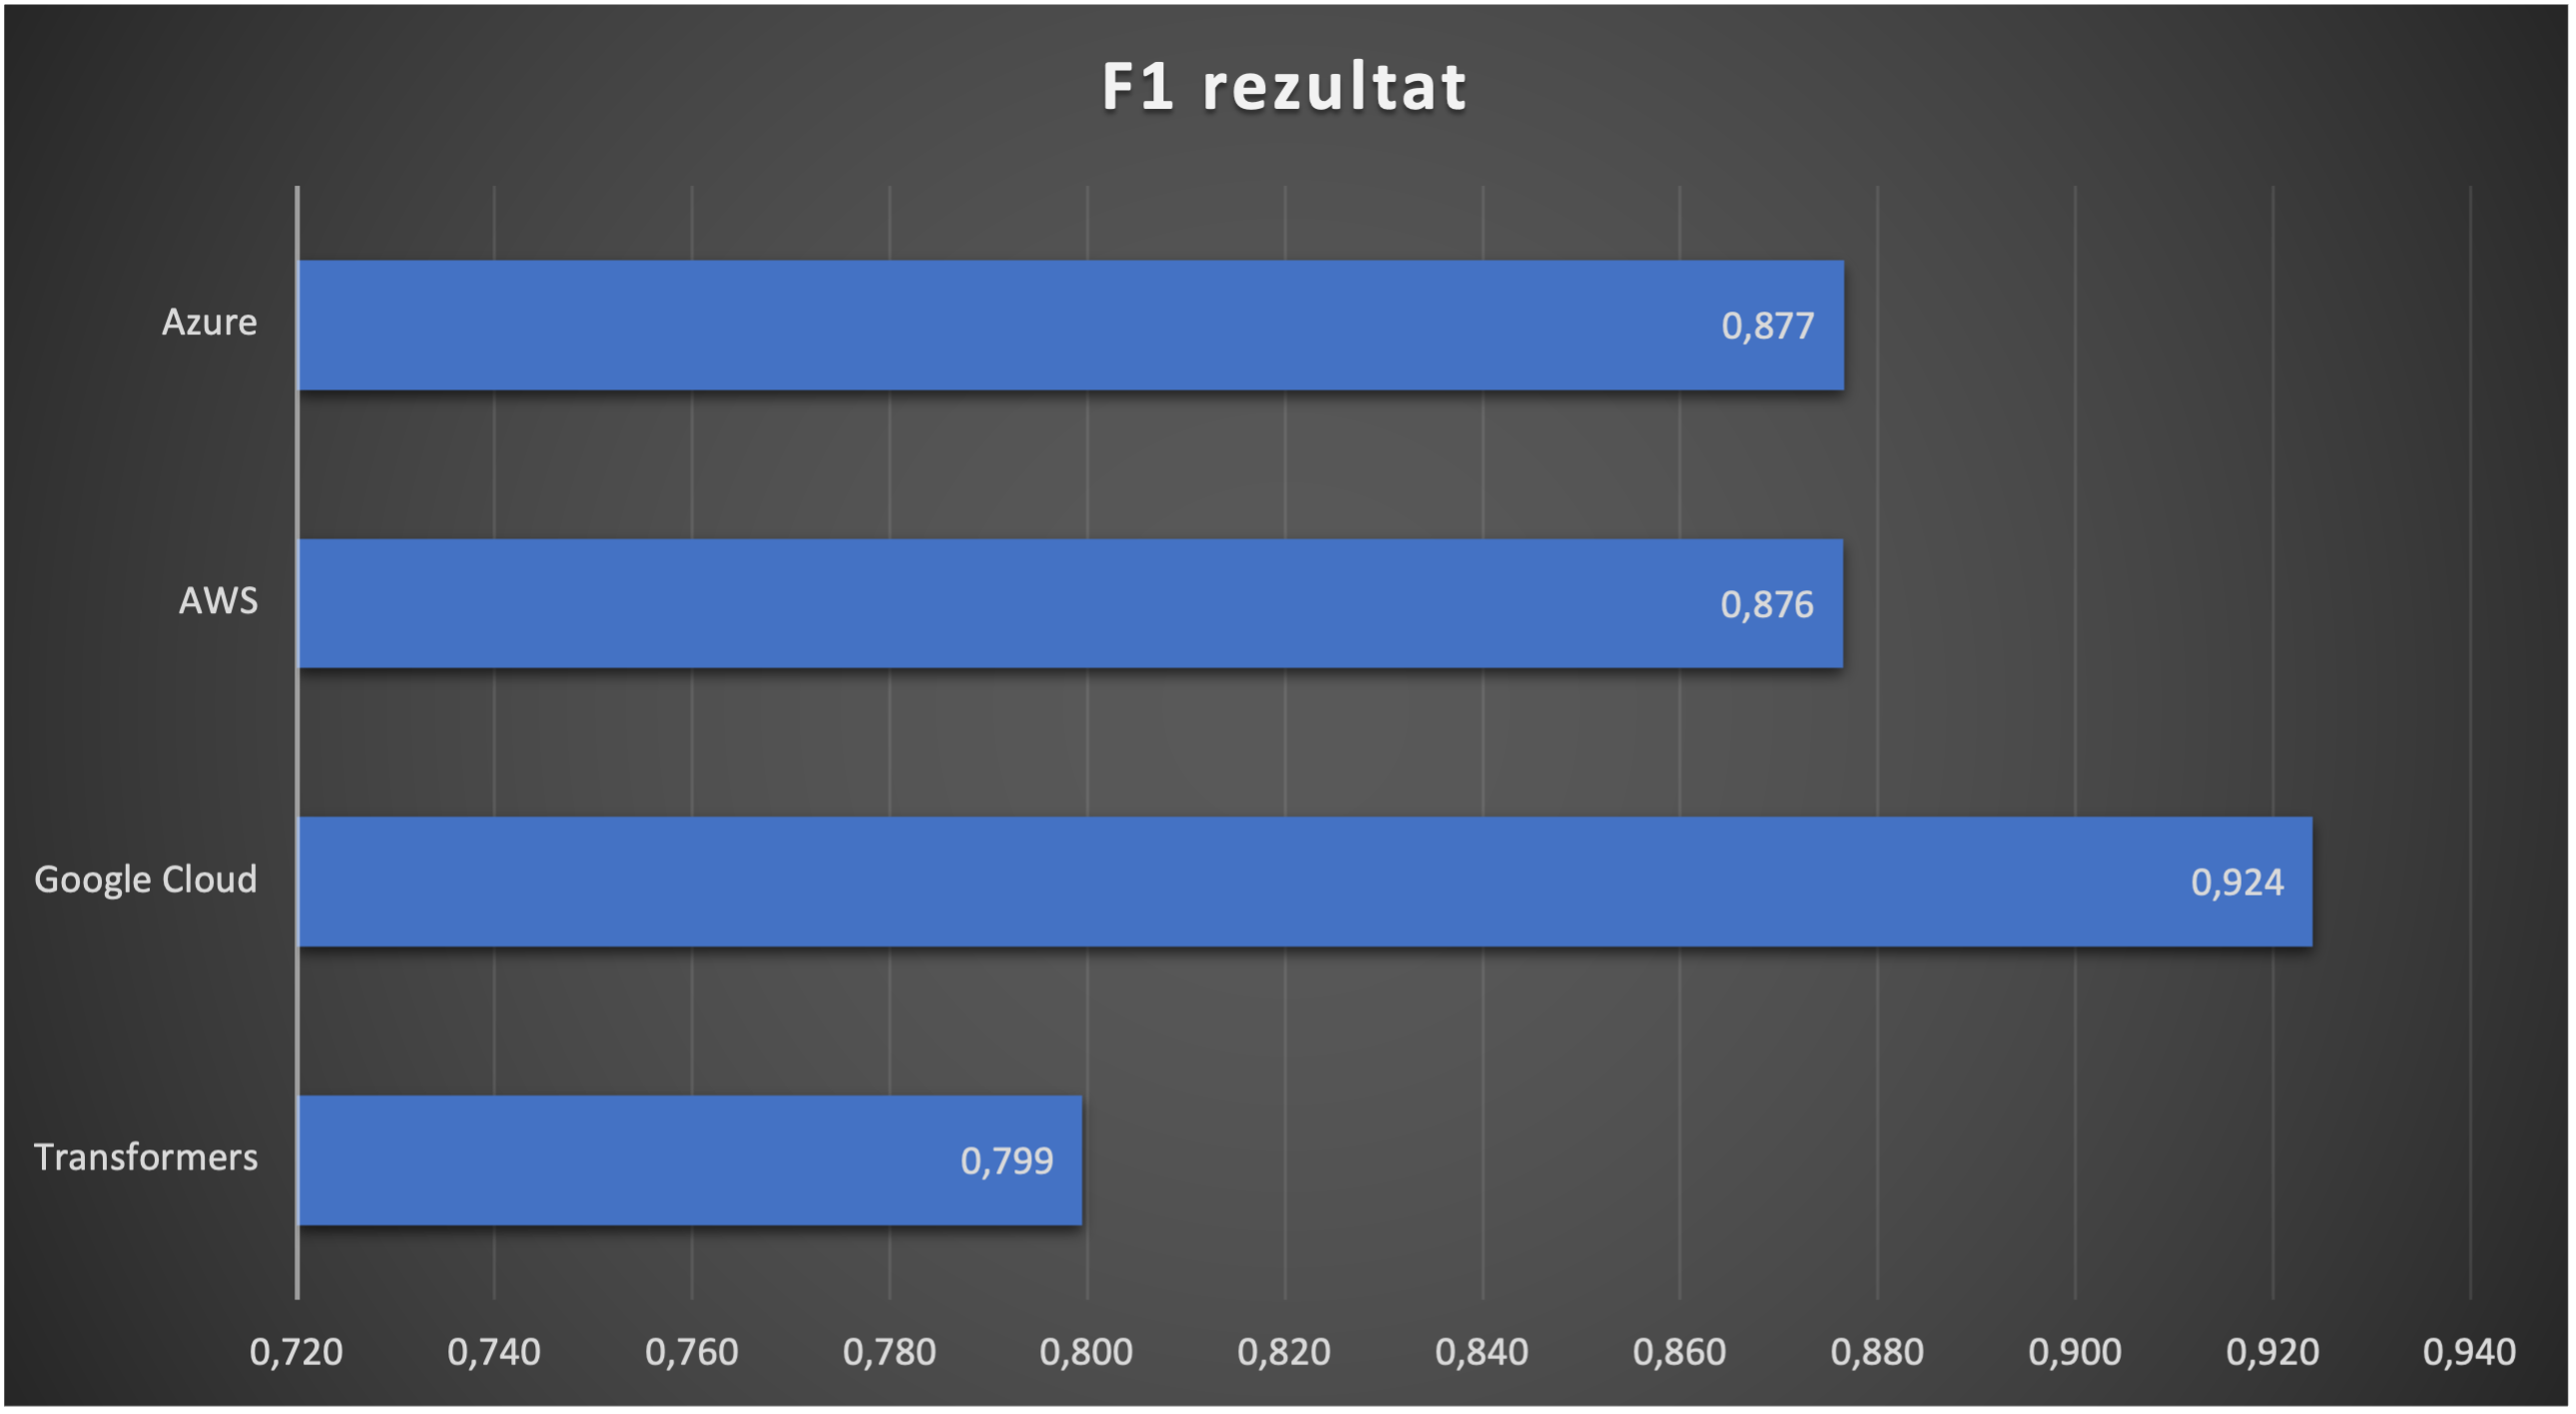
\includegraphics[width=8cm]{KP.png}
\end{center}
\caption{Analiza sentimenta F1 rezultat}
\label{pic2}
\end{figure}
Pri analizi imenskih entitet je bil uporabljen  \hyperref[sec:imdb]{\underline {IMDb Reviews}} dataset.

Za analizo sentimenta  je bila najboljša Vertex AI storitev.

\pagebreak 

\subsection{Povzetek (Summarisation)}
\begin{table}[h!]
\caption{Povzetek }
        \begin{tabular}{l|ccc}
             & {\tt ROUGE-1} & {\tt ROUGE-2}  & ROUGE-L   \\ \hline
                        {\tt Transformers} & 0.209 & 0.190 & 0.192 \\
                        {\tt Vertex AI }   & \textbf {0.429} & \textbf {0.208 } & \textbf {0.306}  \\
                         {\tt AWS SageMaker}   & 0.226 & 0.021 & 0.201 \\     
                        {\tt Azure Cognitive Services}   & 0.426 & 0.220  & 0.330
        \end{tabular}
\label{tbl:1}
\end{table}

 \begin{figure}[h!]
\begin{center}
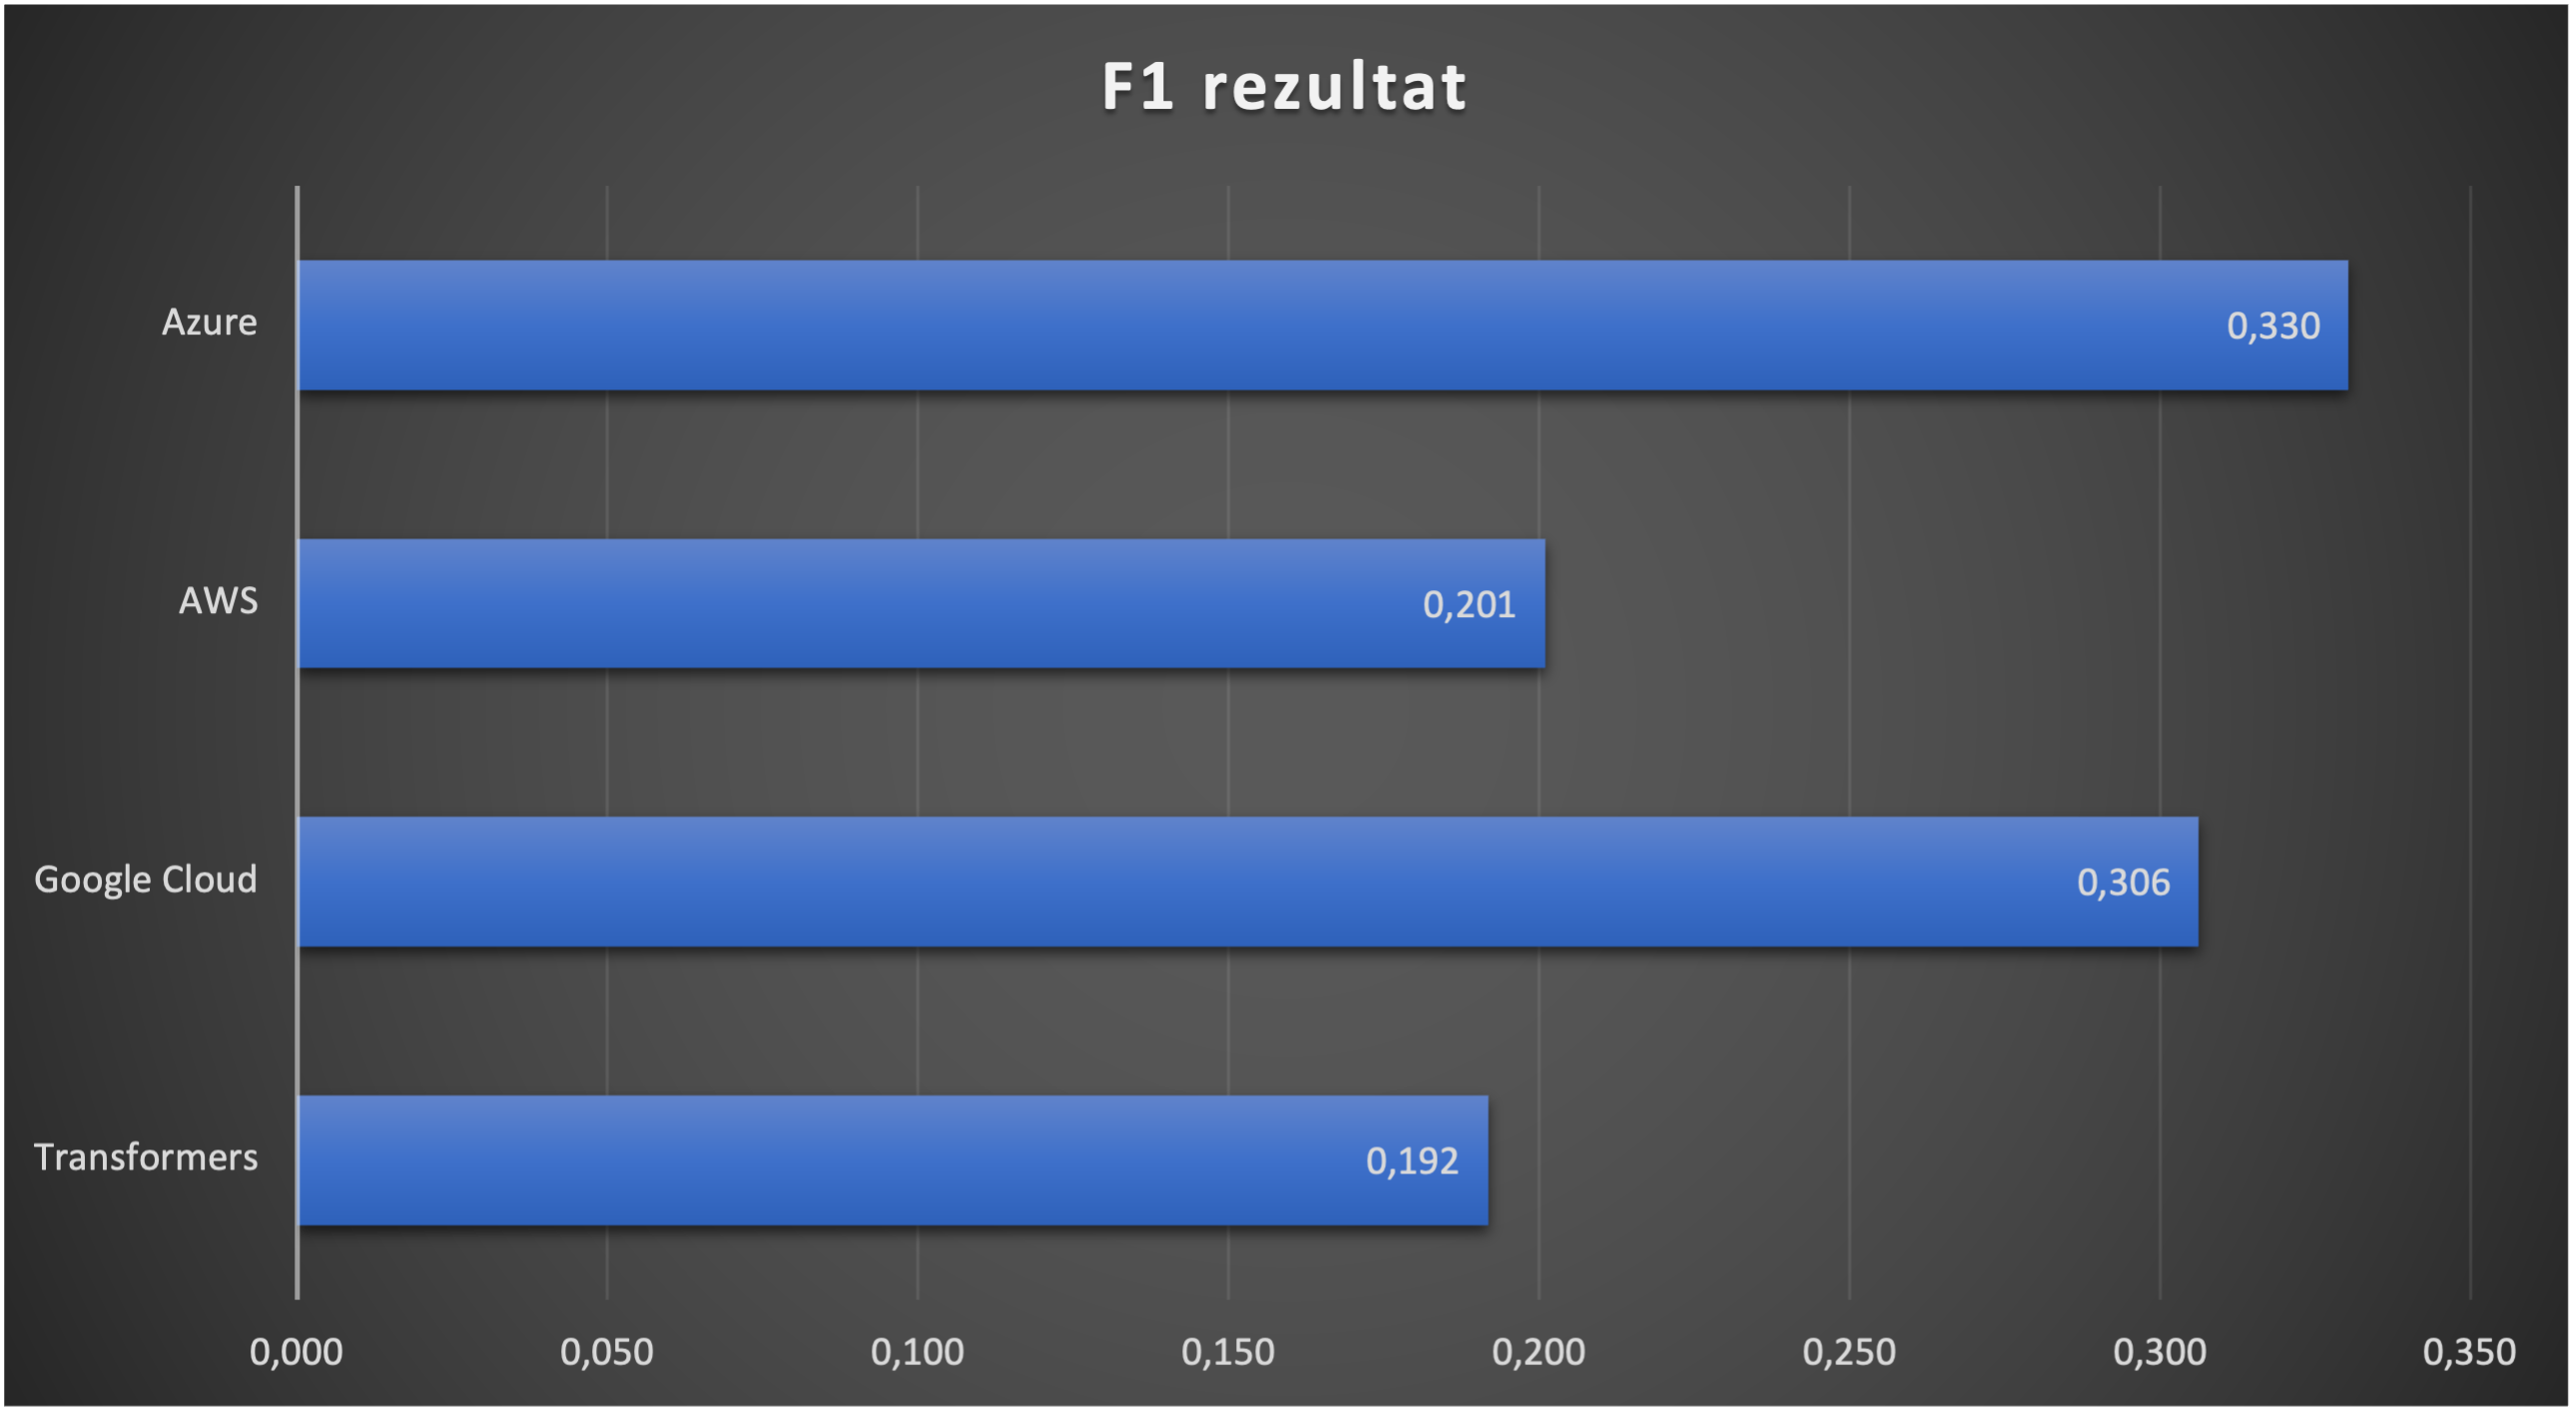
\includegraphics[width=8cm]{SUMM.png}
\end{center}
\caption{Povzetek F1 rezultat}
\label{pic2}
\end{figure}

Pri izdelavi povzetka je bil uporabljen dataset  \hyperref[sec:cnn]{\underline {CNN/Daily Mail}}.

Kot vrhunska izbira za ustvarjanje povzetkov pa se je izkazala storitev Vertex AI.
\pagebreak 
%----------------------------------------------------------------
%Izvleček besedne zveze 

%----------------------------------------------------------------

\subsection{Izvleček besedne zveze  (Key Phrases)}
\begin{table}[h!]
\caption{Izvleček besedne zveze  }
        \begin{tabular}{l|ccc}
             & {\tt Precision} & {\tt Recall}  & F1   \\ \hline
                        {\tt Transformers} & 0.475 & 0.573 & 0.519\\
                        {\tt Vertex AI }   & 0.637 & 0.543  & 0.586  \\
                         {\tt AWS SageMaker}   & 0.513 & 0.622 & 0.562 \\     
                        {\tt Azure Cognitive Services}   &  \textbf {0.530} & \textbf {0.670}  & \textbf {0.592}
        \end{tabular}
\label{tbl:1}
\end{table}

 \begin{figure}[h!]
\begin{center}
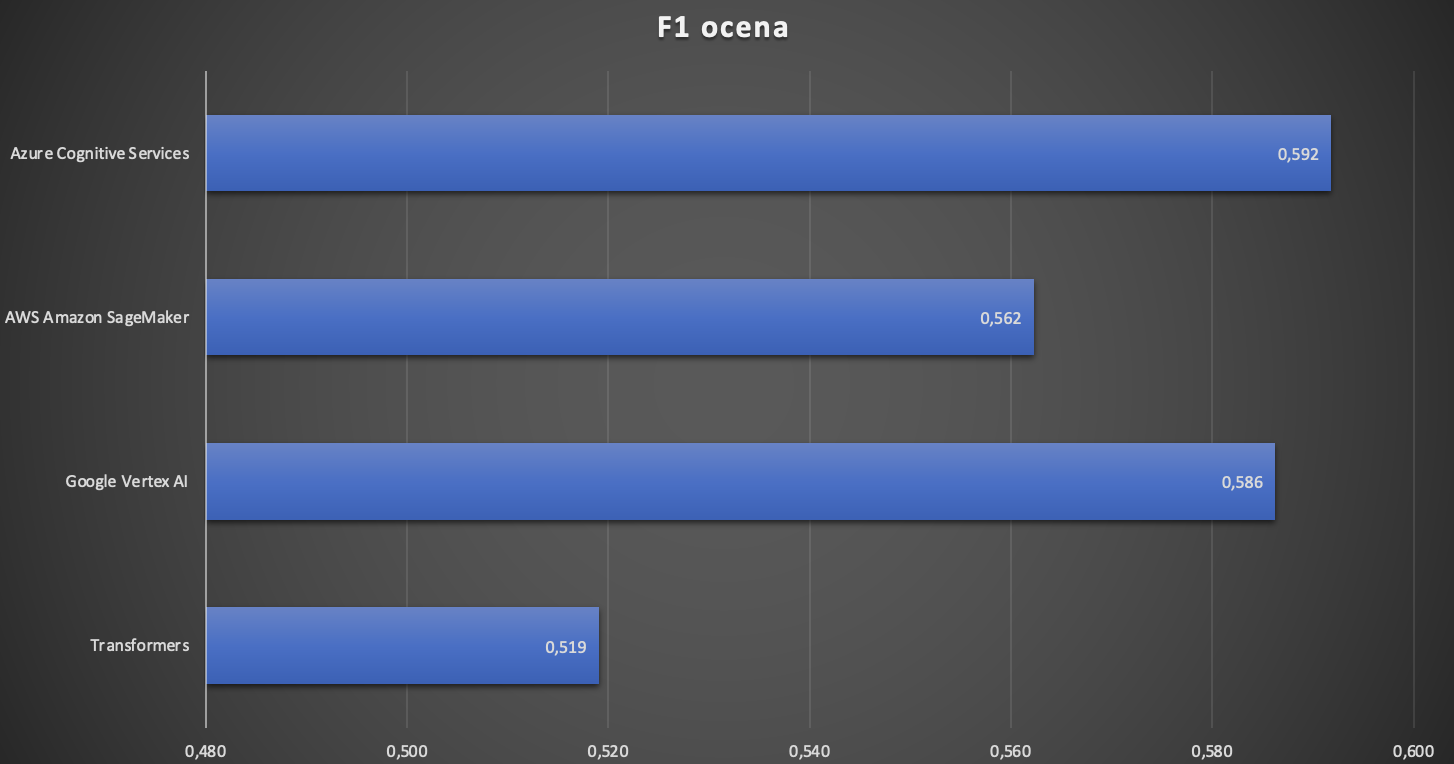
\includegraphics[width=8cm]{KEY.png}
\end{center}
\caption{Izvleček besedne zveze F1 rezultat}
\label{pic2}
\end{figure}

Pri izvajanju naloge zvlečka besedne zveze je bil uporabljen podatkovni niz  \hyperref[sec:semeval]{\underline {semeval-2017}}.

Kot najboljša rešitev za naloge izvlečka besedne zveze pa se je izkazala storitev Azure Cognitive Services.

\pagebreak 
%----------------------------------------------------------------
% Klasifikacija besedila 
%----------------------------------------------------------------

\subsection{Klasifikacija besedila  (Text Classification)}
\begin{table}[h!]
\caption{ Klasifikacija besedila  }
        \begin{tabular}{l|ccc}
             & {\tt Precision} & {\tt Recall}  & F1   \\ \hline
                        {\tt Transformers} & \textbf {0.930} & \textbf {0.926} & \textbf {0.928} \\
                        {\tt Vertex AI }   & 0.957 & 0.862  & 0.907  \\
                         {\tt AWS SageMaker}   & 0.858 & 0.763 & 0. 807\\     
                        {\tt Azure Cognitive Services}   & 0.880 & 0.920  & 0.900
        \end{tabular}
\label{tbl:1}
\end{table}

 \begin{figure}[h!]
\begin{center}
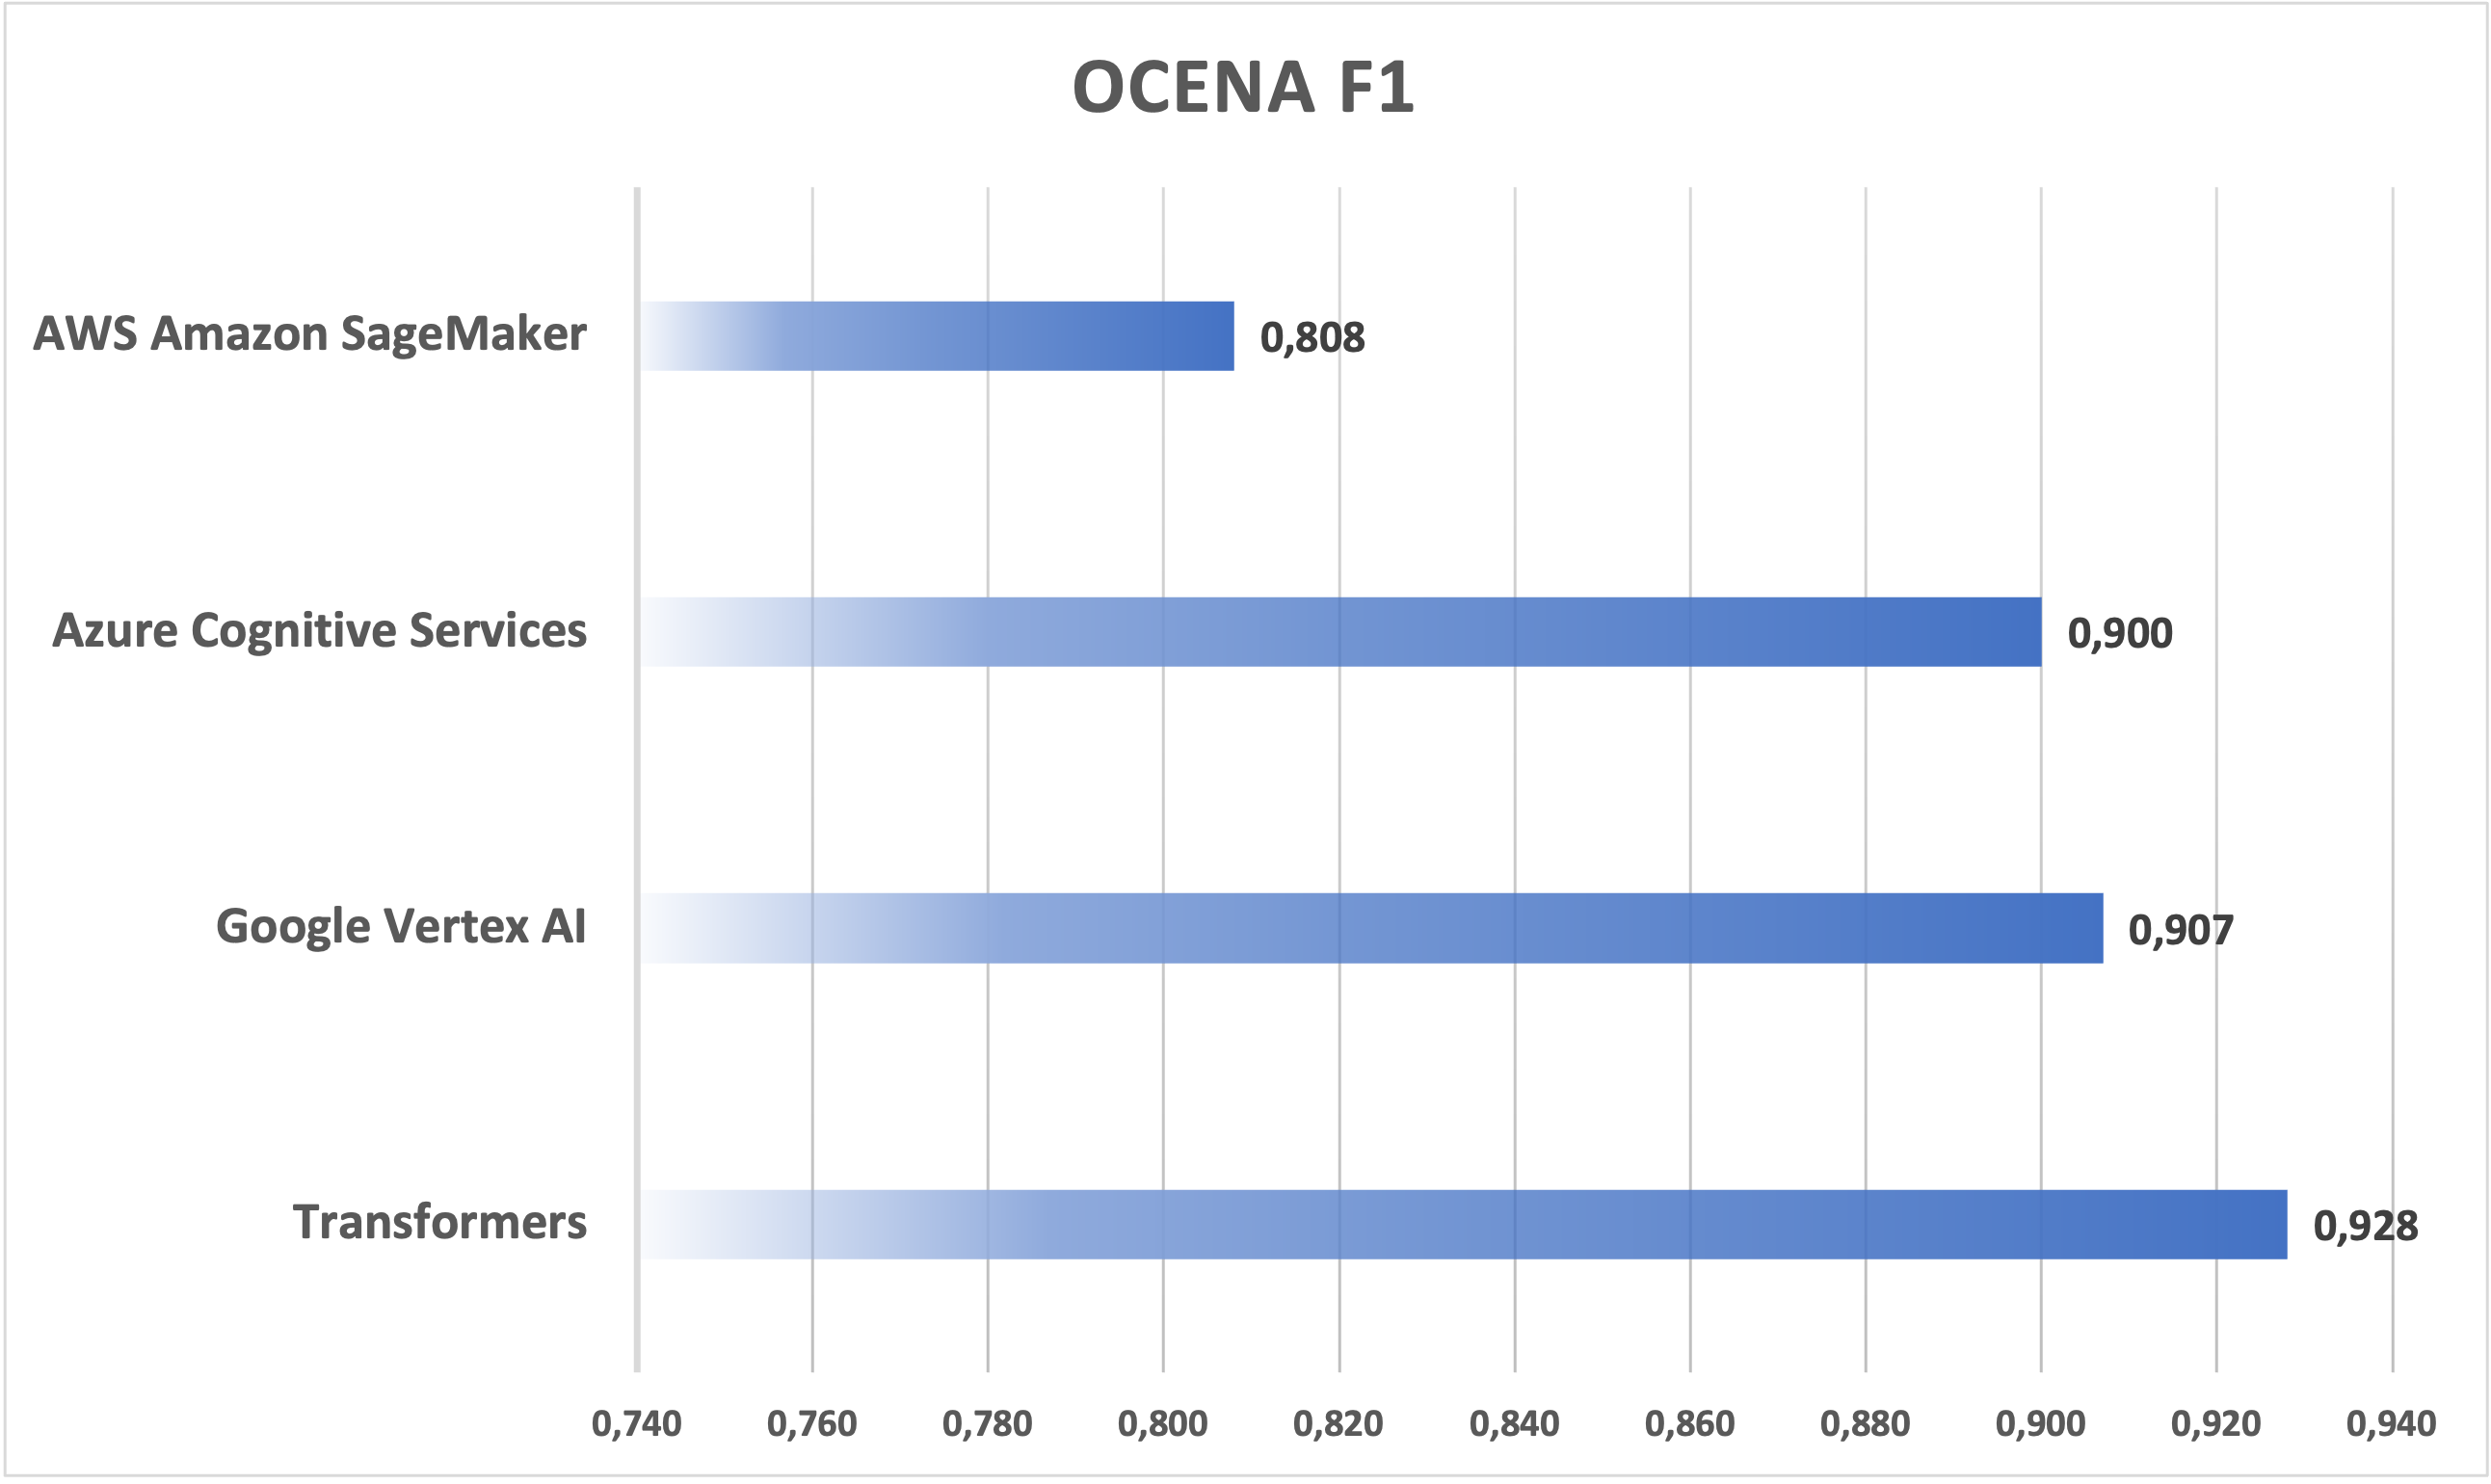
\includegraphics[width=8cm]{CLASSIFICATION.png}
\end{center}
\caption{ Klasifikacija besedila  F1 rezultat}
\label{pic2}
\end{figure}

Pri izvajanju naloge klasifikacije besedila je bil uporabljen podatkovni niz  \hyperref[sec:imdb]{\underline {IMDb Reviews}}.

Kot najboljša rešitev za naloge klasifikacije besedila pa se je izkazala storitev Transformers.

\pagebreak 
%----------------------------------------------------------------
% Zaznava objektov 
%---------------------------------------------------------------

\subsection{Zaznava objektov  (Object Detection)}
\begin{table}[h!]
\caption{ Klasifikacija besedila  }
        \begin{tabular}{l|ccc}
             &  Accuracy   \\ \hline
                        {\tt Transformers} & 0.968\\
                        {\tt Vertex AI }   & 0.977   \\
                         {\tt AWS SageMaker}   & \textbf {0.980}  \\     
                        {\tt Azure Cognitive Services}   &  0.965
        \end{tabular}
\label{tbl:1}
\end{table}

 \begin{figure}[h!]
\begin{center}
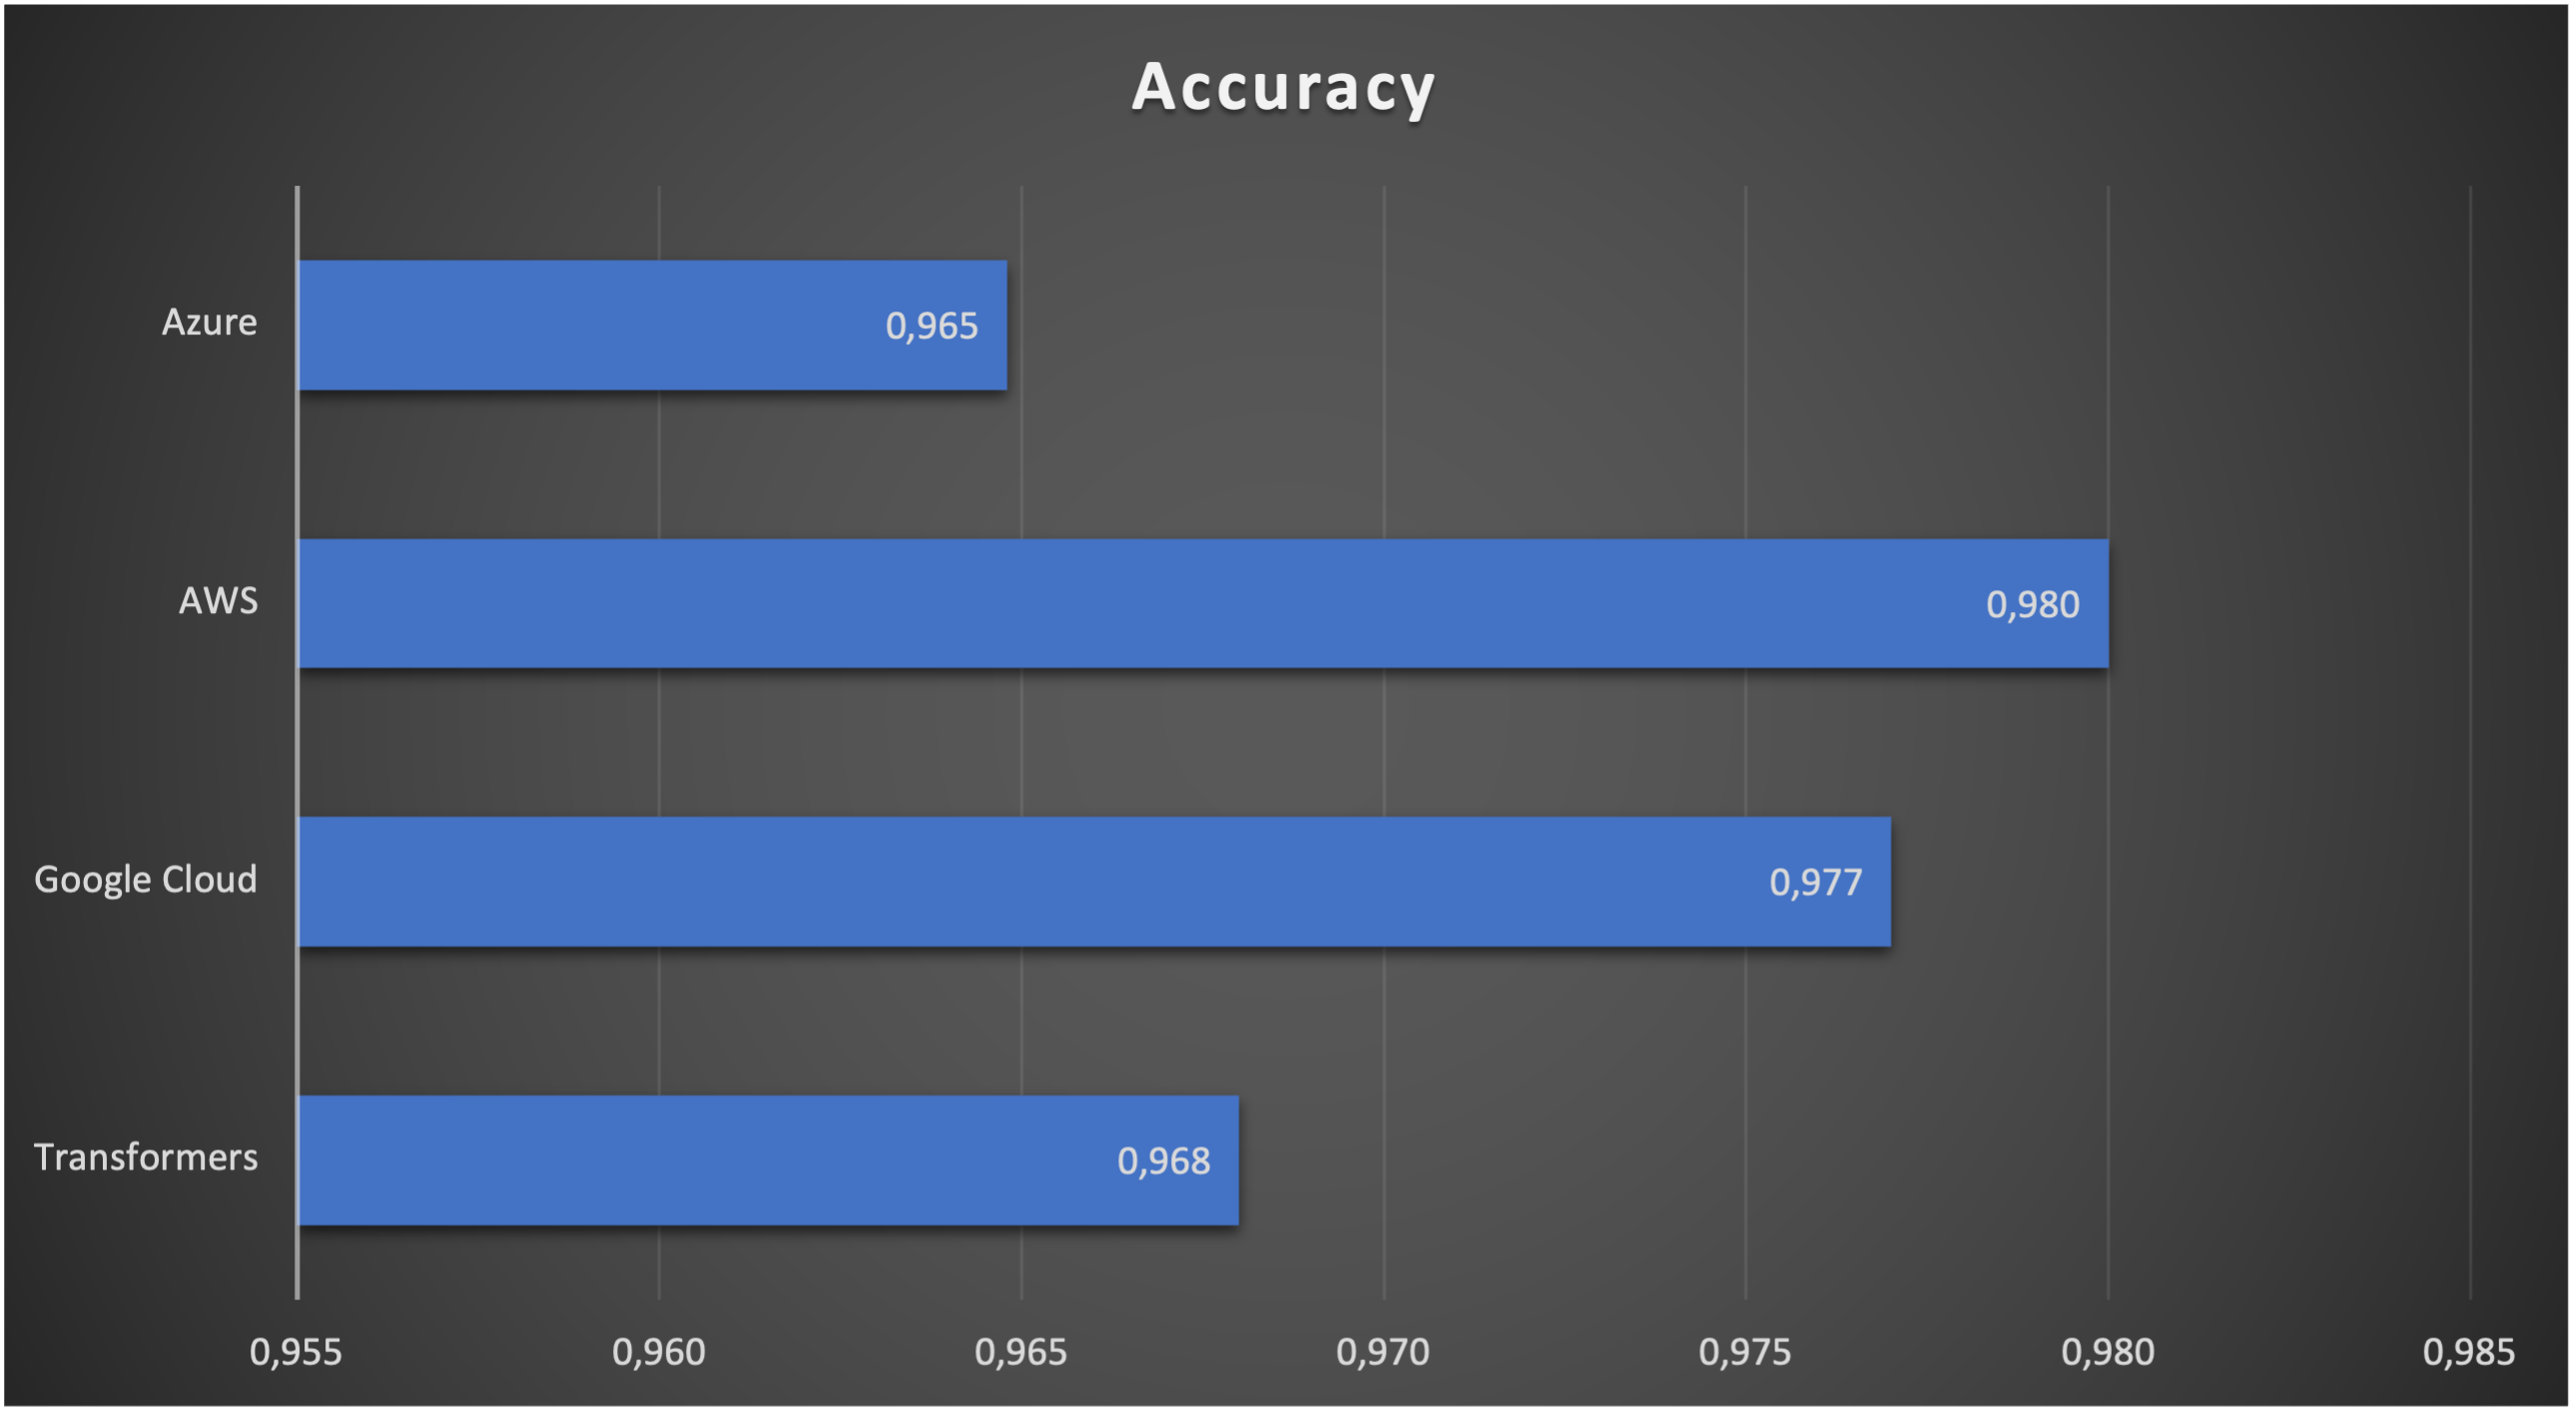
\includegraphics[width=8cm]{OBJECT.png}
\end{center}
\caption{ Zaznava objektov Accuracy rezultat}
\label{pic2}
\end{figure}


Pri zaznavi objektov je bil uporabljen  \hyperref[sec:coco]{\underline {COCO}} dataset.

Kot najboljša izbira za zaznavanje objektov pa se je izkazala storitev AWS SageMaker.


%----------------------------------------------------------------
% Poglavje (Chapter) 6
%----------------------------------------------------------------
\chapter{Sklepne ugotovitve}
Izbira \LaTeX\ ali ne \LaTeX\ je seveda prepuščena vam samim. Res je, da so prvi koraki v \LaTeX{}u težavni. Ta dokument naj vam služi kot začetna opora pri hoji.

% ---------------------------------------------------------------
% Appendix
% ---------------------------------------------------------------
\appendix
%\addcontentsline{toc}{chapter}{Razširjeni povzetek}
\chapter{Title of the appendix 1}

Example of the appendix.

%----------------------------------------------------------------
% SLO: bibliografija
% ENG: bibliography
%----------------------------------------------------------------
\bibliographystyle{elsarticle-num}

%----------------------------------------------------------------
% SLO: odkomentiraj za uporabo zunanje datoteke .bib (ne pozabi je potem prevesti!)
% ENG: uncomment to use .bib file (don't forget to compile it!)
%----------------------------------------------------------------
%\bibliography{bibliography}

%----------------------------------------------------------------
% SLO: zakomentiraj spodnji del, če uporabljaš zunanjo .bib datoteko
% ENG: comment the part below if using the .bib file
%----------------------------------------------------------------

\begin{thebibliography}{99}
\bibitem{Fortnow} L.\ Fortnow, ``Viewpoint: Time for computer science to grow up'',
{\it Communications of the ACM}, št.\ 52, zv.\ 8, str.\ 33--35, 2009.
\bibitem{Knuth} D.\ E.\ Knuth, P. Bendix. ``Simple word problems in universal algebras'', v zborniku: Computational Problems in Abstract Algebra (ur. J. Leech), 1970, str. 263--297.
\bibitem{Lamport} L.\ Lamport. {\it LaTEX: A Document Preparation System}. Addison-Wesley, 1986.
\bibitem{ubi} O.\ Patashnik (1998) \BibTeX{}ing.
Dostopno na: \url{http://ftp.univie.ac.at/packages/tex/biblio/bibtex/contrib/doc/btxdoc.pdf}
\bibitem{licence} licence-cc.pdf. Dostopno na: \url{https://ucilnica.fri.uni-lj.si/course/view.php?id=274}
\end{thebibliography}

\end{document}
